\documentclass[12pt,a4paper]{article}
\usepackage{blindtext}
\usepackage{graphicx}
\usepackage[utf8]{inputenc}
\usepackage[margin=0.65in]{geometry}
\usepackage{multicol}
\usepackage{wrapfig}
\usepackage[dvipsnames]{xcolor}
\usepackage{framed}
\usepackage[most]{tcolorbox}
\usepackage{pgfgantt}
\usepackage{tikz}
\usetikzlibrary{arrows.meta}
\usepackage[dvipsnames]{xcolor}
\definecolor{aliceblue}{rgb}{0.94, 0.97, 1.0}
\colorlet{shadecolor}{aliceblue}
\setlength\parindent{0pt}
\usepackage{charter}
\usepackage{environ}
\usepackage{tikz}
\usetikzlibrary{calc,matrix}
\usetikzlibrary{positioning,fit,calc}
\usepackage{float}
\usepackage{url}
\usepackage{pifont}
\usepackage{tabularx}
\providecommand*{\checkmark}{\textcolor{ForestGreen}{\ding{51}}}
\providecommand*{\xmark}{\textcolor{BrickRed}{\ding{55}}}
% code by Andrew:
% http://tex.stackexchange.com/a/28452/13304
\makeatletter
\let\matamp=&
\catcode`\&=13
\makeatletter
\def&{\iftikz@is@matrix
	\pgfmatrixnextcell
	\else
	\matamp
	\fi}
\makeatother

\lstset{basicstyle=\footnotesize\ttfamily,breaklines=true}
\lstset{framextopmargin=0pt,frame=bottom}
\lstset{backgroundcolor = \color[rgb]{0.98,0.98,0.98}}
\lstset{numbers=left}

\newcounter{lines}
\def\endlr{\stepcounter{lines}\\}

\title{COMPSCI 702 - Security for Smart-devices}
\date{Semester 1, 2018}
\begin{document}
\maketitle
\tableofcontents{}

\section*{Disclaimer}
\textit{This study guide is based off the lecture slides prepared for CS702. It is provided as-is and may contain errors, though effort has been made to minimize this. This resource is not exhaustive and may not contain additional content not covered by the slides.}
\newpage

\section{Access Control}
\subsection{Security objectives}
\begin{shaded}
\begin{itemize}
	\item \textbf{Confidentiality.} Protection of the data.
	\item \textbf{Integrity.} Ensure data is not altered by unauthorized parties.
	\item \textbf{Availability.} Ensure timely access to data.
	\item \textbf{Authentication.} Identify whether communicating entity is who it claims to be.
	\item \textbf{Authorization.} Regulate access to data.
\end{itemize}
\end{shaded}
\subsection{Access control requirements}
The inputs need to be \textit{reliable}, with authenticated entities or genuine information. The \textbf{principle of least privileges} grants the minimum set of access rights to do a job. Furthermore, only a special entity (administrator) can manage (grant/revoke/update) access rights.
\subsection{Elements of access control}
\begin{shaded}
\begin{itemize}
	\item \textbf{Subject.} An entity that can access objects. It can be a user or a process representing a user or an application.
	\item \textbf{Object.} An entity (file, directory, resource) that needs to be protected.
	\item \textbf{Access right.} An access right $r \in R$ describes how a subject $s \in S$ can access an object $o \in O$. Examples include: read, write, execute, create, delete, search, etc.
	\item \textbf{Access control function $f(s, o, r)$} looks up the access right $r$ for combination $(s, o)$. It grants access on a successful match.
	\item \textbf{Security administrator.} Entity that manages access rights.
	\item \textbf{Auditor.} Entity that inspects whole authorization system.
\end{itemize}	
\end{shaded}
\subsection{Access control models}
There are 5 main models for access control:
\begin{itemize}
	\item Discretionary access control (DAC),
	\item Mandatory access control (MAC),
	\item Role-based access control (RBAC),
	\item Usage control (UCON), and
	\item Policy-based access control (PBAC).
\end{itemize}
\subsubsection{Discretionary access control}
Users can protect what they own. The owner can grant access to subjects. Access is granted based on the identity of the requester. These mechanisms are adequate for honest users, but are vulnerable to Trojan horses.\\

DAC is used in operating systems and DBMS. An example is Linux file permissions: \texttt{rwxr-x--x}.

\subsubsection*{Access control matrix}
\begin{shaded}
\begin{center}
\begin{tabular}{lllll}
                            & File 1                                                                            & File 2                                                                            & File 3                                                                            & File 4                                                                          \\ \cline{2-5} 
\multicolumn{1}{l|}{User A} & \multicolumn{1}{l|}{\begin{tabular}[c]{@{}l@{}}owner\\ read\\ write\end{tabular}} & \multicolumn{1}{l|}{}                                                             & \multicolumn{1}{l|}{\begin{tabular}[c]{@{}l@{}}owner\\ read\\ write\end{tabular}} & \multicolumn{1}{l|}{}                                                           \\ \cline{2-5} 
\multicolumn{1}{l|}{User B} & \multicolumn{1}{l|}{read}                                                         & \multicolumn{1}{l|}{\begin{tabular}[c]{@{}l@{}}owner\\ read\\ write\end{tabular}} & \multicolumn{1}{l|}{write}                                                        & \multicolumn{1}{l|}{read}                                                       \\ \cline{2-5} 
\multicolumn{1}{l|}{User C} & \multicolumn{1}{l|}{\begin{tabular}[c]{@{}l@{}}read\\ write\end{tabular}}         & \multicolumn{1}{l|}{read}                                                         & \multicolumn{1}{l|}{}                                                             & \multicolumn{1}{l|}{\begin{tabular}[c]{@{}l@{}}own\\ read\\ write\end{tabular}} \\ \cline{2-5} 
\end{tabular}
\end{center}
An \textbf{access control list}	is a list of access rights on an object. A \textbf{capability list} refers to a user's permissions on different objects. In the diagram, columns are ACLs and rows are capability lists.
\end{shaded}
\subsubsection{Mandatory access control}
MAC restricts access on the basis of security labels. Entities cannot enable other entities to access their resources. Users have security clearance, and resources have security labels that contain data classification.\\

This model is used when information classification and confidentiality are very important, such as in the military. The \textbf{Bell-LaPadula model} (BLP) is used in the US Department of Defence. The \textbf{Biba model} is implemented in the FreeBSD MAC policy. A combined version is used in Android.

\subsubsection*{Bell-LaPadula model}
Goal: Control \textbf{confidentiality of information}.
\begin{itemize}
	\item \textbf{Simple security property.} No read up.
	\item \textbf{*(Star)property.} No write down.
	\item \textbf{Strong *(star)property} No write down and no write up.
\end{itemize}

\subsubsection*{Biba integrity model}
Goal: Control \textbf{integrity of information}.
\begin{itemize}
	\item \textbf{Simple integrity axiom.} No read down.
	\item \textbf{*(Star)-integrity axiom.} No write up.
\end{itemize}
\subsubsection{Role-based access control}
RBAC maps roles to access rights. Supports complex access control. Reduces administrative errors. Flexible to move users or permissions in/out of roles. Least privilege; restrict access according to needs.

\subsubsection*{RBAC model}
\begin{shaded}
\begin{itemize}
	\item \textbf{User.} A human being. Usually. They are assigned roles (\textbf{user assignment, UA}).
	\item \textbf{Permissions.} Approval of a mode of access to some object. They represent what operations could be performed on objects.
	\item \textbf{Roles.} Job title. Roles are assigned permissions (\textbf{permission assignment, PA}).
	\item \textbf{Assignments.} User-role and role-permission.
	\item \textbf{Session.} Mapping between user and an activated subset of assigned roles.
	\item \textbf{Constraints.} Constraintsd are present on sessions, assignments, and roles.
\end{itemize}	
\end{shaded}

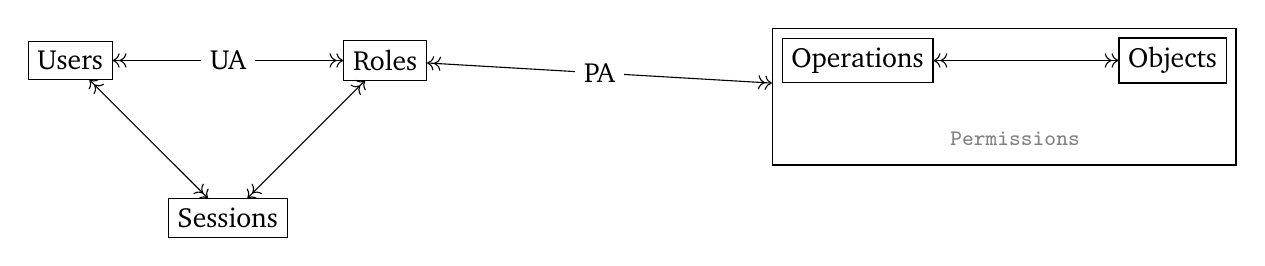
\begin{tikzpicture}[title/.style={font=\fontsize{8}{8}\color{black!50}\ttfamily}]
\node (h) at (12, 1) [title] {Permissions};
\node (a) at (0, 2) [rectangle, draw] {Users};
\node (b) at (4, 2) [rectangle, draw] {Roles};
\node (c) at (2, 0) [rectangle, draw] {Sessions};
\node (d) at (10, 2) [rectangle, draw] {Operations};
\node (e) at (14, 2) [rectangle, draw] {Objects};
\node (f) at (8, 2) [rectangle, draw, fit={(h) (d) (e)}] {};
\draw [<<->>] (a) -- (b) node [midway, fill=white] {UA};
\draw [<<->>] (a) -- (c);
\draw [<<->>] (b) -- (c);
\draw [<<->>] (b) -- (f) node [midway, fill=white] {PA};
\draw [<<->>] (d) -- (e);
\end{tikzpicture}

\subsubsection*{Controlling usage of resources}
DAC, MAC, and RBAC are concerned with checking access rights of entities. Once the access is granted, no more control is enforced.

\subsubsection{Usage control}
UCON doesn't just regulate access to an object, but also focuses on controlling usage. Addresses DRM. DAC, MAC, and RBAC can be expressed by UCON.

\subsubsection*{UCON model}
\begin{shaded}
\begin{itemize}
	\item \textbf{Subjects.} Entities that perform actions.
	\item \textbf{Objects.} Entities accessed by subjects.
	\item \textbf{Rights.} Set of actions.
	\item \textbf{Authorization.} Functional predicates that have to be evaluated for usage decision.
	\item \textbf{Obligations.} Functional predicates that verify mandatory requirements that must have been performed by subject.
	\item \textbf{Conditions.} Environmental/system based decision factors (time, status, etc.)
\end{itemize}	
\end{shaded}
\subsubsection{Policy-based access control}
In PBAC, an authorization policy governs access rights of subjects over objects. Policies are specified independently of entities. This provides a coherent view of access control in a system, and a separation between AC logic and enforcement mechanism.\\

An approach is XACML.

\subsubsection*{PBAC entities}
\begin{itemize}
	\item \textbf{Policy administrator.} Administrates access policies.
	\item \textbf{Policy administration point (PAP).} Interface for policy administration.
	\item \textbf{Policy store.} Repository to store policies.
	\item \textbf{Subject.} Entity that makes access requests.
	\item \textbf{Resources.} Target objects requested by subject.
	\item \textbf{Policy enforcement point (PEP).} Enforces access policies and grants access to resources.
	\item \textbf{Policy decision point (PDP).} Evaluates access policies.
	\item \textbf{Policy information point (PIP).} Provides contextual information.
\end{itemize}
\section{Android Security}
\subsection{Introduction to Android}
Android is a smartphone (open-source) OS currently developed by Google based on the Linux kernel. The SDK was released in November 2007 for Java, followed by the NDK (native development kit) in June 2009 for C and C++. The \textbf{Open Handset Alliance} is a consortium of 84 firms for developing open standards for mobile devices.\\

Android \textbf{fragmentation} is a problem. Vendors can customize the OS for their own devices by including their own apps. Some of these apps may compromise security/privacy as they have technical vulnerabilities. Vendors also might not push updates as frequently, and leave devices a few versions behind. Some vendors stop supporting their devices afterwards as well. \textit{The lack of support can lead to vulnerabilities.}\\

Android is considered \textbf{middleware} between the Linux kernel and its set of APIs. Android apps are mainly written in Java, and only Android apps can run on Android devices. Through the APIs, apps can access device information/components.

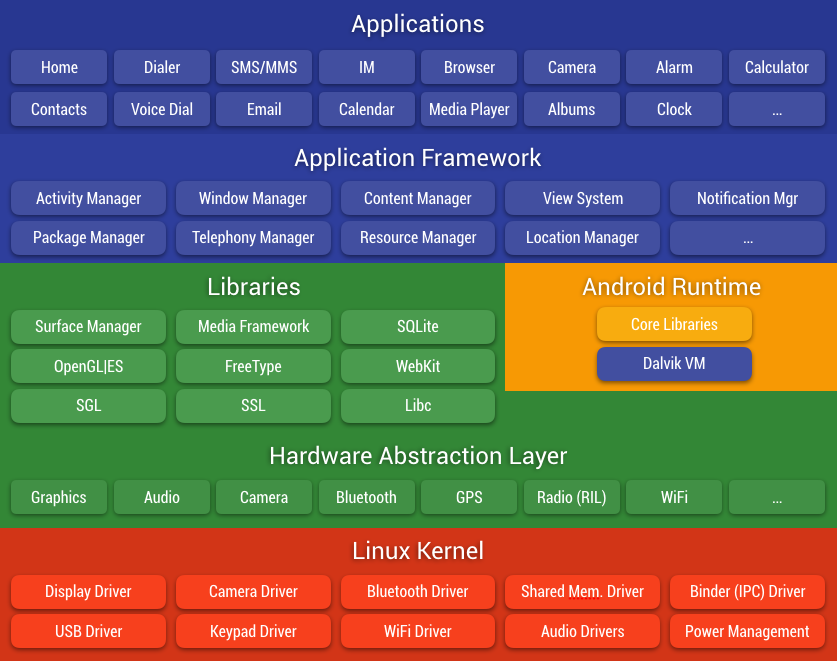
\includegraphics[width=\textwidth]{graphics/androidanatomy}

\paragraph{Linux kernel}
Android is built on the Linux kernel\footnote{It is \textbf{not} Linux.}. There is no \texttt{glibc} support, nor does it include the full set of Linux utilities. There are some kernel enhancements.\\

The Linux kernel was chosen as it has great memory/process management. It also has a permissions-based security model, a proven driver model, support for shared libraries. The Linux kernel is also open-source.

\paragraph{Binder}
Applications and services may run in separate processes but must communicate and share data. \textbf{Issue:} Inter-process communication (IPC) can introduce significant processing overhead and security holes. \textbf{Solution:} Driver to facilitate IPC.

\paragraph{Power management}
Mobile devices run on battery power with limited capacity. The power management features are built on top of Linux power management, but has more aggressive power management policy.

\subsubsection*{Native libraries}
Bionic \texttt{libc} is a custom \texttt{libc} implementation.\\

Why Bionic? \texttt{glibc} is licensed under LGPL, which prevents static linking of proprietary software. The size needs to be small as it will load in each process, and needs to be efficiency due to limited CPU power. \textbf{Bionic \texttt{libc}} is under the BSD license, is small, and efficient due to a custom pthread implementation. It does not support some POSIX features, is not compatible with \texttt{glibc}, and all native code must be compiled against Bionic.

\subsubsection*{Hardware abstraction layer}
This layer is a user-space C/C++ layer which separates the Android platform logic from the hardware interface.\\

A user-space HAL is necessary as 1) not all components have standardized kernel driver interfaces; 2) kernel drivers are licensed under GPL, which exposes any proprietary IP; and 3) Android has specific requirements for hardware drivers.

\subsubsection*{Android runtime}
\paragraph{Dalvik VM}
Android's custom clean room implementation. Provides application portability and runtime consistency. This runs Dalvik bytecode (optimized file format \texttt{.dex}). Java \texttt{.class}/\texttt{.jar} files are converted to \texttt{.dex} at build time.\\

The VM is also designed for embedded environment. It supports multiple virtual machine processes per device. It has a highly CPU-optimized bytecode interpreter, and uses runtime memory very efficiently.

\paragraph{Core libraries}
These are Core APIs for Java which provide a powerful and simple/familiar development platform. They are basically Java wrappers around C/C++ based libraries.

\subsubsection*{Application framework}
These are services essential for Android. Apps don't access them directly.

\subsubsection*{Applications}
These are applications.

\subsubsection{Runtime}
At startup, the bootloader loads the Linux kernel and starts the \texttt{init} process. The \texttt{init} process starts the \textbf{zygote} process, a nascent process that initializes a Dalvik VM instance. It forks on request to create VM instances for managed processes. It uses copy-on-write to maximize re-use and minimize footprint. \textit{There is an instance of DalvikVM per APK.}\\

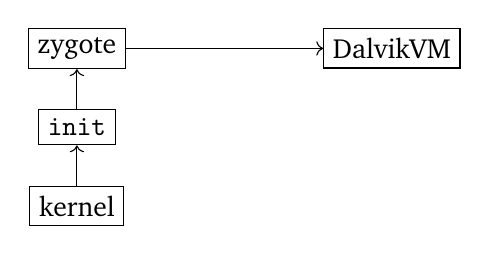
\begin{tikzpicture}[title/.style={font=\fontsize{8}{8}\color{black!50}\ttfamily}]
\node (a) at (0, 0) [rectangle, draw] {kernel};
\node (b) at (0, 1) [rectangle, draw] {\texttt{init}};
\node (c) at (0, 2) [rectangle, draw] {zygote};
\node (d) at (4, 2) [rectangle, draw] {DalvikVM};

\draw [->] (a) -- (b) node [midway] {};
\draw [->] (b) -- (c) node [midway] {};
\draw [->] (c) -- (d) node [midway] {};
\end{tikzpicture}

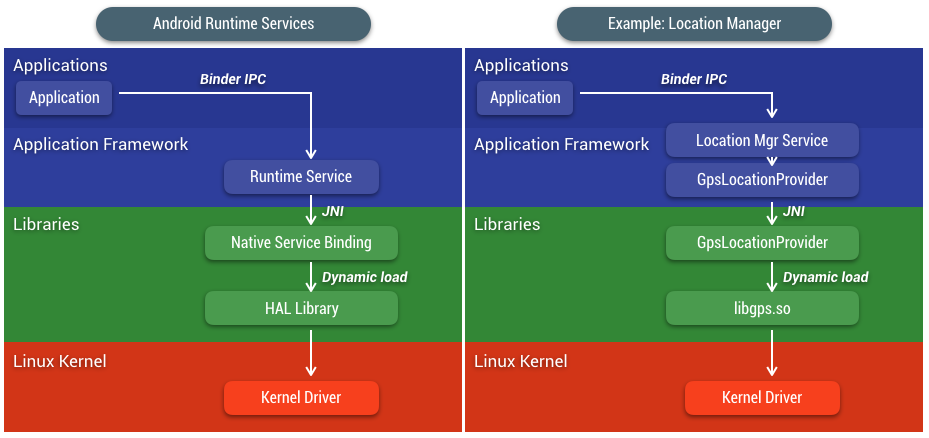
\includegraphics[width=\textwidth]{graphics/androidrt}

\subsubsection*{Android security objectives}
The goals are to protect user data, protect system resources (+network), and provide application isolation. 

\begin{shaded}
\textbf{Key Android security features:}
\begin{itemize}
	\item Robust security at OS level through Linux kernel
	\item Mandatory app sandboxing for all applications
	\item Secure IPC
	\item Application signing
	\item Application-defined and user-granted permissions
\end{itemize}	
\end{shaded}

\subsection{Android application model}
The Android application package (APK) consists of the following components:
\begin{itemize}
	\item \textbf{\texttt{classes.dex}.} Dalvik executable of Android app components
	\item \textbf{Resources and assets.} Images, string values, raw data, layouts, etc.
	\item \textbf{Native code.} C/C++ shared libraries linked dynamically
	\item \textbf{META-INF.} Certificate and signature information
	\item \textbf{Application manifest.} XML file that declares app metadata/components (names, intent filters, permissions). Its main elements are package info, app info (icon, etc.), activity component, etc.
\end{itemize}

Android requires that all apps be digitally signed with a certificate. Android apps used self-signed certificates. This certificate is used to identify the developer of an app. Android follows the \textbf{same-origin policy}. Android uses the same signing key-pair to ensure that updates come from the same developer.\\

An Android app is a combination of loosely coupled components. Each component can offer multiple entry points.
\begin{itemize}
	\item Activity: user interface
	\item Service: background services
	\item Content provider: database
	\item Broadcast receiver: mailbox for broadcasted messages
\end{itemize}

\subsubsection*{Intents}
\textbf{Intents} are named events and represent the \textit{intent} to do something, such as launching an activity, starting service, or broadcasting a message. Its payload and attributes describe the intended action. It can be sent/received by an app.\\

An \textbf{explicit} intent sets the target component name, such as \texttt{com.example.app.MainActivity}.\\

An \textbf{implicit} intent provides information including action, data, and type. This is resolved at runtime by the package manager. The Android framework will find a suitable receiver for this intent. For example: \texttt{Action=intent.ACTION\_VIEW; Data=www.youtube.com} will open an app that can show YouTube, such as the YouTube app or the default web browser.

\subsubsection*{Activity}
\begin{wrapfigure}{r}{0.5\textwidth}
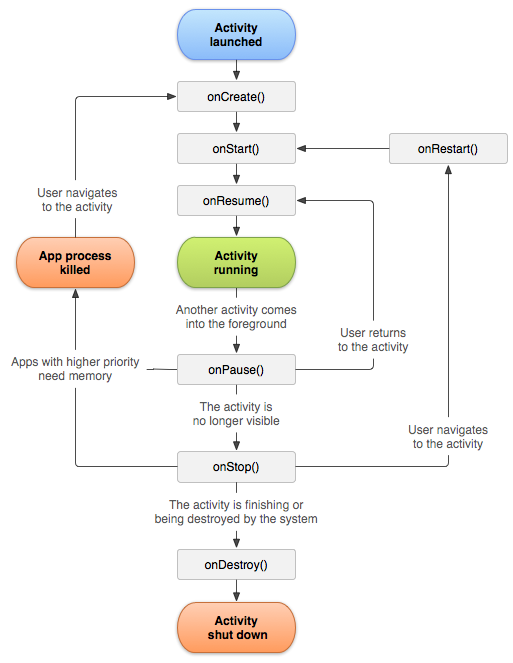
\includegraphics[width=0.5\textwidth]{graphics/activity_lifecycle}
\end{wrapfigure} 
An \textbf{activity} is a main building block of GUI applications. It is like a website; multiple activities represent multiple ``pages'', and the main activity is like the homepage. It is possible to move from an activity to another, just like navigating through pages.\\

There are system calls as state changes due to user actions. If there is another activity started, the on-going activity is paused. App process may be killed, and a stopped activity can be destroyed.\\

The \textbf{Activity Manager} is responsible for creating, destroying, and managing activities. When a user starts an application for the first time, the AM will create its activity and put it onto the screen. When the user switches screens, the AM will move the previous activity to a holding place, so if the user wants to go back to an older activity it can be started more quickly.\\

Older activities that haven't been used for a while will be destroyed to free space for current ones.

\subsubsection*{Service}
A \textbf{service} is a background process without a user interface, used to perform some long-running operation, such as downloading files or playing music. It can be local to the app or provided by other apps. Services can define a remote interface using the Android Interface Definition Language. The AIDL compiler creates skeleton for implementation of the service (stub). Services are started and stopped on demand.\\

App components start unbounded services. A \textbf{bounded service} acts as a server. The app component (client) logs in (binds) to the server, consumes the services, and then unbinds.\\

Use an \textbf{unbounded service} to do work if the app components don't need interaction with the service again. Use a \textbf{bounded service} if interaction is required.


\subsubsection*{Content providers}
\textbf{Content providers} are interfaces for sharing data between apps. The interfaces are simple: \texttt{select(), insert(), update(),} and \texttt{delete()}. They must be declared in the manifest with the \texttt{<provider>} tag.\\

Content providers are accessed by the URI \texttt{content://<authority>/<resource>}.\\

\paragraph{Contacts} Content provider that exposes user contact data to applications. The contacts app uses the contacts provider (a separate app) to retrieve contacts data. The contacts app does not have contacts data.

\paragraph{Settings} Exposes system settings to applications, including to Settings.

\paragraph{Media} Store responsible for storing/sharing media across applications.

\subsubsection*{Broadcast receiver}
A \textbf{broadcast receiver} is a component that responds to system-wide events. It's a mailbox for broadcast intent messages. Intent filters can be defined to indicate what messages to receive.\\

Events can come from the system (SMS, low battery), or an application (data update complete).\\

Broadcast receivers are Android's implementation of a system-wide publish/subscribe mechanism. The system or apps are publishers, and user apps are subscribers. A subscribing app can subscribe by indicating intent filters in the manifest or registering dynamically. The receiver will receive a triggered event if there is a subscription.\\

Events are broadcasted to a number of receivers who subscribe for the event.\\

A BR has to register with the Activity Manager and the Package Manager. This can be done through the manifest or programmatically\footnote{I highly doubt code details are examinable...}.
\begin{shaded}
\begin{lstlisting}
<receiver android:name=``MsgListener''>
   <intent-filter>
      <action android:name=``compsci702.intent.action.BROADCAST''/>
   </intent-filter>
</receiver>
\end{lstlisting}

The \texttt{MsgListener} class is responsible for processing the intent. The \texttt{<action>} tag specifies the intents to be received.\\

To do it programmatically, add an intent with \texttt{IntentFilter\#addAction()} and override \texttt{onReceive(Context c, Intent i)} for the action to be performed, then register the receiver and filter.

\end{shaded}
\begin{figure}[h]
\centering
\caption{Android build process}
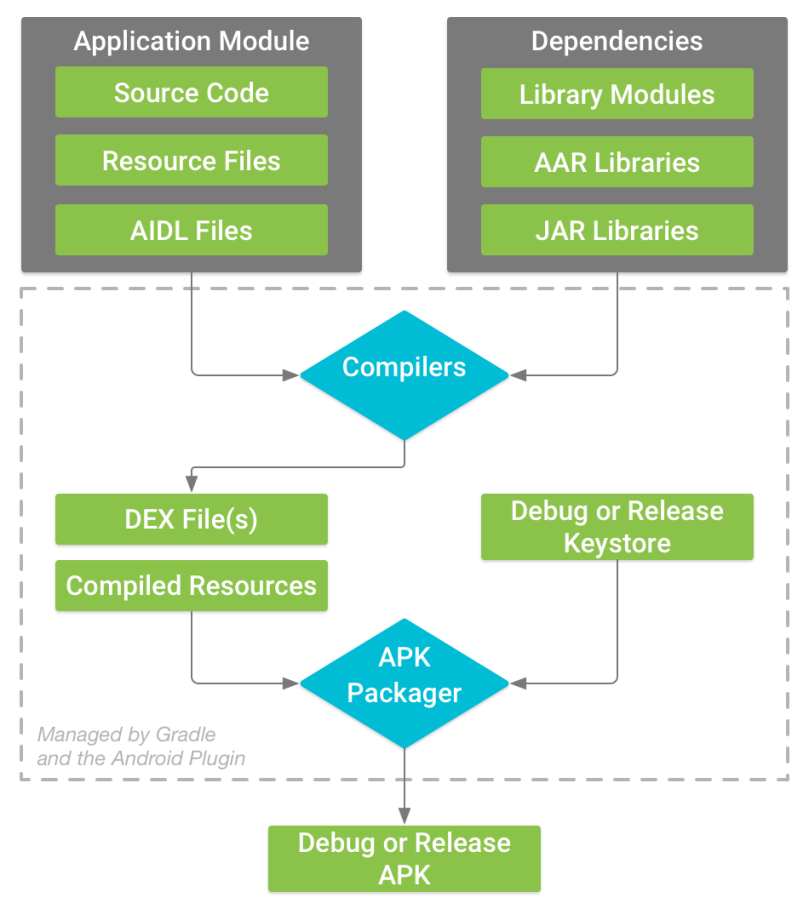
\includegraphics[width=0.5\textwidth]{graphics/build-apk}
\end{figure}

\subsection{Android ICC}
\subsubsection*{Android Binder}
Binder enables \textbf{inter-component communication} (ICC) in Android. It is implemented as a Linux kernel driver, as a customized version of Open Binder. It provides a simple RPC-like mechanism. Apps use Java methods to invoke ICC, then Android translates this into C++ invocations and system calls to the binder driver.\\

In Linux, processes communicate and share data through pipes, shared memory, and message queues. In Android, app components communicate through binder.\\


The \textbf{Activity Manager} is a service that apps use for ICC. It provides over 100 methods, including these common ones: \texttt{startActivity()}, \texttt{startBroadcast()}, \texttt{startService()}, and \texttt{bindService()}. Apps export services by publishing them through the Activity Manager.\\

The \textbf{Service Manager} is a special system service to keep track of available services. An app that wants to provide a service to others can publish its service through the Service Manager. Communication to the Service manager takes place through the Binder.\\

The Service Manager accepts these commands:
\begin{itemize}
	\item \textbf{Publish.} Used to publish a service within the Service Manager. Takes arguments: service name and address.
	\item \textbf{Get/check.} Returns an address of the service in form of handler. Takes argument: service name.
	\item \textbf{List.} Lists the service names registered with the Service Manager.
\end{itemize}

The Android middleware contains a \textbf{reference monitor} that mediates the establishment of ICC. This is part of the Activity Manager.

\subsubsection*{MAC security enforcement}
A reference monitor enforces MAC for regulating access to app components. Access to each component is restricted by assigning it an access permission label. Applications are assigned collections of permission labels. When a component initiates ICC, the reference monitor checks if its permission label is same as the target component's access permission label.\\

The Android middleware implements a reference monitor providing MAC enforcement about how apps access components.

\begin{figure}[h!]
\centering
\caption{A's ability to access B and C is determined by comparing the access permission labels on B and C with the collection of labels assigned to App 1.}
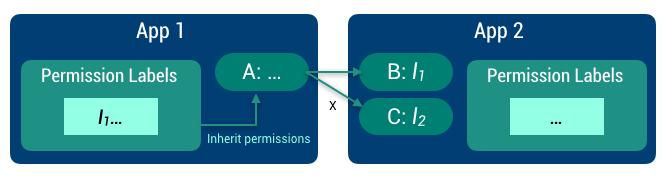
\includegraphics[width=0.9\textwidth]{graphics/plabels}
\end{figure}

Assigning permission labels to an app specifies its protection domain. Android's policy enforcement is mandatory: permission labels can't be changed until the app is reinstalled. This model restricts access to components and doesn't provide information flow guarantees.

\subsection{Sandboxing}
\textbf{Sandboxing} specifies which system resources an application is allowed to access. This limits malicious apps to perform actions only in the sandboxed environment. \\

There are two levels of sandboxing:
\begin{itemize}
	\item \textbf{Process level.} Each application is run in a dedicated process and access to sensitive resources depends on permissions. \begin{itemize} 
	\item Android assigns a unique User ID (UID) to each Android app.
	\item A UID (AppID) is generated at install time.
	\item It runs each app as a separate process with its UID.
	\item Apps run within the sandboxing environment in the kernel.
	\end{itemize}
	\item \textbf{Filesystem level.} Each application has its own private data directory and only the application can access its own data directory. \begin{itemize} 
	\item Each app is assigned a dedicated data directory.
	\item This applies to all apps (even native apps).
	\item Only the app has permission to read/write to its data directory.
	\end{itemize}
\end{itemize}

The app data directory is implemented based on Linux DAC. Permissions are set by the system \texttt{rwxrwxrwx}. Only the owner/root can change permissions.\\

System daemons and apps run under well-defined/constant UIDs. The root has UID 0. System UIDs are statically defined in the \texttt{android\_filesystem\_config.h} header file.\\

UIDs for system services start from 1000:
\begin{itemize}
	\item \texttt{android.uid.phone} (PHONE\_UID, 1001)
	\item \texttt{android.uid.bluetooth} (BLUETOOTH\_UID, 1002)
	\item \texttt{android.uid.log} (LOG\_UID, 1007)
	\item \texttt{android.uid.nfc} (NFC\_UID, 1027)
\end{itemize}

Apps can be installed using the same UID. Apps can share files and run in the same process. Shared UIDs are used by system apps which use the same set of resources. (Example: in Android 4.4, the system UI and keyguard share the same UID).\\

Shared UIDs aren't recommended for non-system apps, but is still available as long as the apps are signed with the same signing key.

\subsection{Permissions}
Apps are sandboxed, so they can only access their own files. Android can grant additional access rights (permissions) to apps. This helps Android control access to resources.\\

Apps request permissions defined in \texttt{AndroidManifest.xml}. Apps can request a set of additional permissions granted at runtime. A user may be asked to grant requested permissions. Android comes with a built-in list of pre-defined permissions. When new features come out, associated permissions are added as well. \textbf{Custom permissions} can be defined by system and user-installed apps.\\

An app that wants to receive incoming SMS (\texttt{RECEIVE\_SMS}) has to declare:

\begin{lstlisting}
<uses-permission android:name="android.permission.RECEIVE_SMS"/>
\end{lstlisting}

\subsubsection*{Permission management}
Permissions are assigned to each app by the package manager, which maintains a central database of installed packages with info about install path, version, certificate info, assigned permissions to each package, and a list of all permissions defined on a device. This database is in \texttt{/data/system/package.xml} and is updated every time an app is installed, updated, or uninstalled.

\subsubsection*{Permission protection levels}
The levels characterize potential risk in the permission and indicate the procedure that the system should follow when determining whether to grant the permission.

\begin{itemize}
	\item \textbf{Normal.} This is not security critical and is granted without asking users. \begin{itemize} \item\texttt{ACCESS\_NETWORK\_STATE} allows apps to access network information.\end{itemize}
	\item \textbf{Dangerous.} Grants access to user data or some control over the device. Involves functionalities that can cost money, so requires user approval. \begin{itemize}
	\item \texttt{READ\_SMS} allows apps to read SMS.
	\item \texttt{CAMERA} gives apps access to camera.
	 \end{itemize}
	 \item \textbf{Signature.} Only granted to requested apps that are signed with the same key as the app that declared the permission. Strongest permission level as it requires cryptographic key possession. Apps using these permissions are controlled by the same developer. Decided by system without requiring user intervention. Typically used by system apps that do device management.
	\begin{itemize}	 \item \texttt{NET\_ADMIN} allows configuration of network interfaces, IPSec, etc.
	\end{itemize}
	\item \textbf{SignatureOrSystem.} Granted to apps part of the system image or signed with the same key as the app that declared permission. Allows vendors to have pre-installed apps to share specific features that require a permission without having to share signing keys. Until Android 4.3, any app installed in the system partition was granted this permission. Since Android 4.4, apps need to be installed in \texttt{system/priv-app} to get this.
\end{itemize}

\textit{TODO: The diagrams on these slides...}

\subsection{Security refinements}
Android's security framework is based on MAC and DAC. It offers additional refinements as well which are exceptions.

\subsubsection*{Public and private components}
Private components simplify security specification as devs don't have to worry about permission labels. By default, components are public (but declare them as private for best practice).\\

Apps may contain components that others should never access, such as a password. Developers can declare this component private (in manifest file, set exported attribute to false). Private components can only be accessed by other components in the same app.\\

\subsubsection*{Implicitly open components}
Developers frequently define intent filters on activities. For example, the system may find an image viewer when an intent has a \texttt{VIEW} action. The caller won't know beforehand what access permission is required. The developer of the target activity can declare it open by not assigning access permission to it (public without permissions).\\

This default policy specification enables functionality and ease of development. However, any app can have access and can lead to poor security practices.\\

Best practices:
\begin{itemize}
	\item Components must be declared open in exceptional cases.
	\item Consider splitting components to sub-components to specific fine-grained control.
\end{itemize}

\subsubsection*{Broadcast intent permissions}
A broadcast intent is read by all apps so can lead to the leaking of sensitive information. With a broadcast intent permission, the developer can protect the intent. This is declared programmatically with \texttt{sendBroadcast(intent, PERMISSION)}.

\subsubsection*{Content provider permissions}
Always define both read and write permissions for content providers, which provide interfaces for reading and writing.

\subsubsection*{Service hooks}
If a component has the permission, it can start, stop, or bind the service at any time. To specify more flexible and fine-grained access control, Android lets components invoke the \texttt{checkPermission()} method. This is done at the code level.

\subsubsection*{Pending intents}
Pending intents delegate actions to another application. This allows other apps to invoke services on behalf of the requesting app. This allows better integration with third party apps, but since it enables delegation, it deviates from MAC.

\subsubsection*{URI permissions}
Android uses a special content URI to deal with content providers, and can specify a record within a table. An app that doesn't have a read permission to access the content provider can get access with a URI permission. The developer can pass a URI in an intent filter. This also deviates from MAC.

\subsection{Security weaknesses}
Poorly designed apps can result in resources being exposed or depleted, as well as the loss of privacy.

\subsubsection*{Privilege escalation}
An adversary tries to escalate privileges to gain unauthorized access to protected resource.\\

\paragraph{Confused deputy attack} If an app doesn't have a permission, it can ask its neighbor. This leverages the vulnerability in a benign app.
\paragraph{Collusion attack} Multiple apps can collaborate to get permissions which each of them cannot get otherwise. For example, if an app has access to location, and another has access to the internet, they can collude to expose user information on the internet.\\

Android supports all-or-nothing access and doesn't offer fine-grained access control. If an app has access to the internet and contacts, the app can use contacts and use the internet. It is not okay for the app to publish contacts through the internet. \textit{Information flow techniques needed to prevent information disclosure.}

\subsection{Runtime permissions in Android 6}
Android 6.0 Marshmallow was released in October 2015 (API level 23). In this version and onwards, users grant permissions at runtime rather than at install-time. This streamlined the app installation process and also gives user more control over the app's functionality. A user can give a camera app access to the camera but not the location.\\

Users can revoke permissions at any time in the Settings app.\\

From a user's perspective, permissions can be categorized in to normal or dangerous. Normal permissions are automatically granted as they don't risk privacy. Dangerous permissions have to be approved as they can give the app access to confidential data.\\

Prior to Android 6, users had to grant dangerous permissions when they install the app as the app won't be installed if the user doesn't grant permissions. Now, the app lists all the permissions in its manifest, and must request each dangerous permission it needs while the app is running. Users can grant/deny each permission; the app will still run (with limited capabilities).\\

Permissions must be checked each time an operation that requires the permission is called by calling the \texttt{checkSelfPermission()} method. This returns \texttt{PackageManager.PERMISSION\_GRANTED} if the app has the permission, or \texttt{PackageManager.PERMISSION\_DENIED} if it doesn't, at which point the app has to ask the user for permission.\\

With Android, explanations for permissions can be added so that the user can know why a certain permission is required.\\

When an app requests permissions, the system presents a dialog box to the user; the app cannot change the dialog box. When the user responds, the system invokes \texttt{onRequestPermissionsResult()}. The app must override that method to determine if the permission was granted.\\

There are two ways for an app to perform a task: by asking the permission, or use an intent to get another app to perform the task. With permissions, the app has full control over the UX, but this adds complexity to the task. With the use of intents, the app that handles the intent provides the UI and thus the app has no control over the UX.

\subsection{App distribution}
The Google Play Store is Google's app distribution platform and official Android app store. To distribute apps, developers have to pay a registration fee for a Google Play Developer Console account. Developers receive 70\% of the app's price. Only Android devices that comply with Google's compatibility requirements may install and access apps.\\

\textbf{Malware} is software that can disrupt normal activities, such as compromising privacy, reliability, confidentiality, etc. 99\% of mobile malware is on Android.

\paragraph{Spyware} Collect sensitive information and upload to remote servers. Example: FakeNetflix collects Netflix credentials.
\paragraph{Destructive trojans} Modify content on devices. Example: Android.Elite.1.origin is a fake Angry Birds game.
\paragraph{Financial charges} SMS trojan for sending SMS to premium numbers. Example: FakePlayer sends a hard-coded message to premium numbers in Russia.
\paragraph{Ransomware} Steal data or disables phone functionality and asks for money to unlock this data.
\paragraph{Mobile botnets} Receive commands from remote command and control servers.
\paragraph{Root-kit exploits} Lots of stuff.

\subsubsection*{Google Bouncer}
Google Bouncer is an in-house anti-malware system by Google as a first line of defense against Android malware. It emulates Android apps on Google's cloud and looks for anomalies that may be indicative of malware. Full coverage but less reliable.

\paragraph{Static analysis} Analysis that does not require code execution. A static analysis tool inspects programs for possible runtime behaviors to find potentially malicious code.
\paragraph{Dynamic analysis} Requires code execution to determine program flow. Reliable but lacks coverage.

In 2015, a Google announcement announced that the app review process will involve a team of experts.

\subsection{Google Bouncer}
Google Bouncer was easily bypassed. This section discusses how that happened.\\

It was discovered that it was possible to submit apps without paying. Submit a sample app that connects to a command and control server, but do no harm. Bouncer ran the app before it was published.\\

Bouncer did runtime analysis of app in an emulated Android environment for 5 minutes on Google's infrastructure. It allowed external network access.\\

It was possible to fingerprint the QEMU version and get information. The Android ID returned was indicative of an emulator, but recent tests indicate that the ID is now dynamic. The account owner was associated with \texttt{miles.karlson@gmail.com}.\\

In short, Bouncer runs your app for 5 minutes so if you don't do anything bad for 5 minutes it's fine. Bouncer is not a physical device. It explores the app by emulating input and clicking. If your app is flagged, then a human analyzes the app.

\subsection{App installation and scanning}
\textbf{App repackaging} is a major attack vector. Attackers can't forge signatures but can remove the original signature and re-sign the repackaged app with a new certificate. This new app encloses a malicious payload. Android prevents malicious updates but breaks trust on the first time install.\\

Android apps can be installed from the Play Store or via \textbf{sideloading}, or installing apps from other sources. The latter requires enabling installation from \textit{unknown sources} in security settings.\\

Sideloading can take place through USB (e.g. \texttt{adb install app.apk}), Bluetooth, Wi-Fi, third party app stores, or downloads.\\

Google Play offers security services:
\paragraph{Protection within Google Play Store} Play Store has policies in place to protect users from attackers. Developers are reviewed when they create their developer account based on profile and credit cards. They are also reviewed upon app submissions. Google Play also scans apps for malware and other vulnerabilities, and suspends accounts that violate policies.
\paragraph{App review} Ratings and reviews provide information about an app. Apps that mislead users may have low reviews. (What about paid reviews and all that?)
\paragraph{Remote app removal} Google can remove malicious apps the store. If an installed app poses a threat, Google can remotely remove it.
\paragraph{Google Play Protect} This is an additional service that provides protection from apps outside of Google Play. This scans apps when you install them and scans for potentially harmful apps. By default, app verification is enabled but can be disabled. (Can it identify obfuscated harmful apps?)

\subsection{Android for Work}
\textbf{TrustZone} supports a full Trusted Executed Environment (TEE) and runs in a special CPU mode called Secure Mode. Memory for secure mode and security functions are hidden from the ``normal world." Android vendors can supply security features such as secure boot or DRM with this.\\

Cryptography is used throughout Android to ensure confidentiality and integrity. Applications of it include: device encryption, app signing, and network connectivity/encryption.

\subsubsection*{Device encryption}
Process of encoding user data on an Android device with an encryption key. If device encryption enabled, all user-created data automatically encrypted before storing on disk. All reads automatically decrypt data before returning to calling process. Android disk encryption based on \texttt{dm-crypt}. Android uses AAES for device encryption\\

Application security include: sandboxing, permissions, SELinux, app signing, Google Play reviews and Play Protect.\\

\subsubsection*{Network security}
Android provides secure communications over the Internet by supporting TLS/SSL. Their security team developed a tool called \texttt{nogotofail} which confirms if devices/apps are safe against known vulnerabilities/misconfigurations.\\

\subsubsection*{BYOD}
Android 5 and onwards support enterprise use cases.\\

BYOD refers to the policy of allowing employees to bring their own devices to the workplace. They are used to gain privileged corporate information/apps.\\

A primary user is the first user added to a device. They can't be removed unless it's by a factory reset. This user also has special privileges and is always running. Secondary users can be added and removed by the primary user.\\

A \textbf{work profile} is a separate Android user managed by the enterprise. The \textbf{profile owner} can manage the corporate space on a user's personal device. The \textbf{device owner} is like a profile owner but to the device; it is the device admin in the corporate use case.

\subsubsection*{Application management}
\textbf{Google Play for Work} offers APIs used by enterprise mobility management (EMM) vendors to allow them to manage apps. IT admins can remotely install/remove apps on a managed Android for Work device. They can define which users can see which apps, and can see which users have which apps installed.\\

Apps can be published by an enterprise customer and targeted privately. There are two modes of delivery: Google-hosted or externally-hosted. Apps must comply with Google Play policies.\\

An app can allow IT admins to remotely control the availability of features or configure settings.
\newpage
\section{iOS Security}
\subsection{Overview}
Smartphones are always with us. They contain lots of data on them, such as passwords, contacts, and documents. It's likely for them to be lost or stolen. They're always on, and so present a continuous target. They change networks repeatedly, between wireless and cellular networks, resulting in a greater chance of a man-in-the-middle attack. People are less likely to use long passphrases due to keyboard limitations.\\

Smartphones are subject to almost all standard security attacks: malicious sites, Trojan horses, buffer overflow attacks, social engineering, etc.\\

We want to protect the data on the device, data sent/received by the device, our apps, the operating system. We want to make sure the device works properly!

\subsection{Introduction to iOS security}
\subsubsection*{iPhone OS 1.0 (2007)}
iPhone OS 1.0 was a cut down version of OS X and offered very little in terms of security:
\begin{itemize}
	\item No privilege separation. All processes ran as root.
	\item No code signing.
	\item No data execution prevention (DEP)
	\item No address space layout randomization (ASLR)
	\item No sandboxing
\end{itemize}

There was some attempt to reduce the attack surface. It did not support Flash or have a shell. The mobile version of Safari, MobileSafari, did not deal with all formats that Safari could. Its PDF viewer only parses a few features (PDF rendering has still been used in many exploits).


\subsubsection*{iOS 2 onwards}
Security was taken much more seriously. The App Store was introduced in iOS 2 (2008).

\subsubsection*{Users and security}
There is a trade-off of some degree between convenience and security.


\subsubsection*{Passcodes}
Use a passcode. This prevents easy access to others and can be used to encrypt files on device. This should be combined with auto-lock, so attackers would need the passcode to access the device.\\

Use a strong passcode. A delay is enforced after repeated incorrect passcode brute force attempts (up to 1 hour at 9 attempts). Data protection can be enabled so that all data is erased after 10 failed attempts.\\

A separate restriction passcode is available for access to apps (think: parental controls). Every time you leave the Restrictions screen you need to re-enter the passcode.

\subsubsection*{App privileges}
Since iOS 6, the user is asked when apps attempt to use certain services, such as Location Services.\\

These can be considered MAC policies.

\subsubsection*{Mobile phone theft}
\begin{shaded}
\textbf{Find My iPhone} \\
This feature must be set up on device and uses the user's Apple ID. Apple devices can be put into Lost Mode so that a passcode is required to unlock the device. The device is also tracked on a map, and emails are sent when any event happens.\\

All data can be erased by deleting the filesystem encryption key.
\end{shaded}

In iOS 7, Activation Lock was introduced. The Apple ID of the device is stored on Apple's activation servers. Find My iPhone cannot be turned off and the phone can't be erased or reactivated without it.\\

An encrypted backup cannot be restored without the password.

\subsubsection*{Kill switch}
Apple can remotely delete apps on your device. It is not clear if it has been used in the past. Google has it as well and they've used it. This is part of their terms and conditions.

\subsection{iOS device and app trust evaluation}
iOS verifies trusted apps with mandatory \textbf{code signing}. Only apps signed by Apple (or by someone certified by Apple) are installed.\\

The device checks the certificate and signature before running the app. The app code and memory is continually checked as the app runs.\\

Signing involves verifying the signer and the integrity of the app code.\\

When an executable is loaded, the signature is loaded and checked in kernel. If it is \underline{not} in the \textbf{static trust cache}, a function is called to check the signature.\\

Apps that come with the device don't have a signature; the binary's hash is stored in the iOS kernel in the static trust cache.

\subsubsection*{Digital signatures}
\paragraph{Public key cryptography.} A key pair with a public key and a private key. The signer encrypts using the private key.
\paragraph{Hashing} An app digest. The hashes of two different apps are different.\\

\begin{figure}[h]
\centering
\caption{Verifying integrity of an application \textit{(Note: S is the digital signature)}}
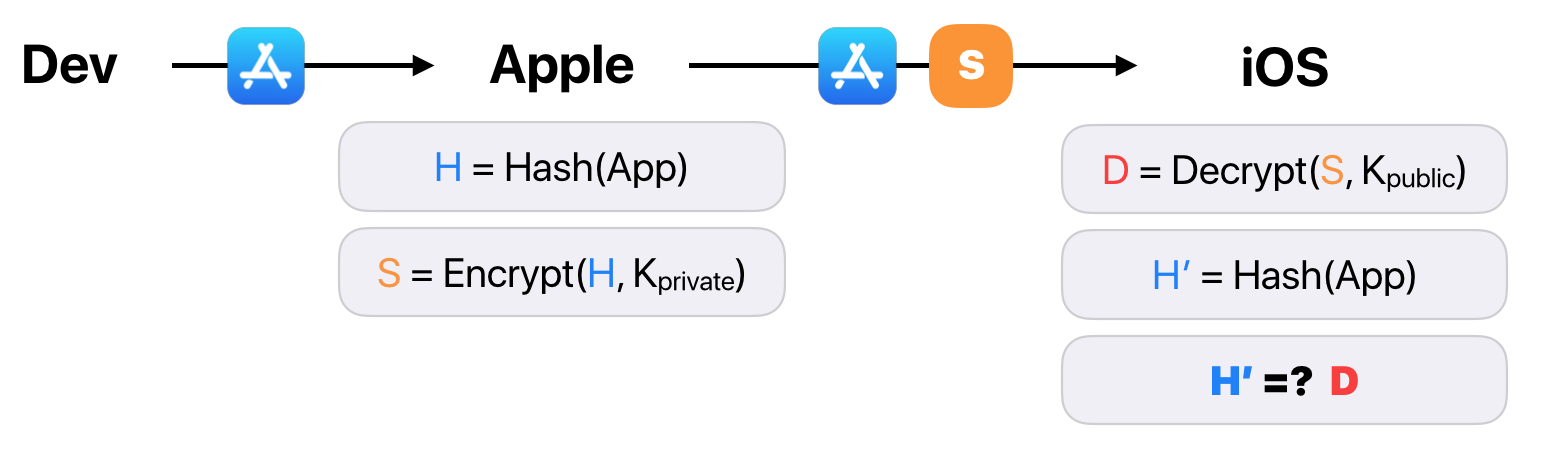
\includegraphics[width=0.9\textwidth]{graphics/iossign}
\end{figure}

The app developer sends an app to Apple who review and sign the application. The \textbf{signature} comprises of encrypting the app hash with Apple's private key. To verify the app, decrypt the signature with Apple's public key and verify that the hashes are the same.\\

\subsubsection{iOS app testing}
\textbf{Problem:} If signing is always required, how can app developers test or debug newly developed apps?

\subsubsection*{Apple provided certificates}
Certify that Alice holds private key of the public key to be used by Bob's iPhone.

Certify that \textit{Alice} holds the private key of the public key to be used by \textit{Bob's} iPhone.\\

Apple provides a \textbf{developer certificate} for app development and a \textbf{distribution certificate} for app distribution.

\begin{shaded}
Certificate = public key(Message) + Apple's digital signature
\end{shaded}

\subsubsection{Provisioning Profiles}
\paragraph{Provisioning profile} An XML property list (plist) required for an app that is being developed to be installed on a certain device. It configures the device to allow the execution of signed code. It is installed on the device only if the device ID is in the profile.\\

The plist describes which app (App ID; random characters followed by company ID/name), which devices (each device has a 40-char hex unique device ID), developer certificate, and entitlements.\\

\textbf{Entitlements} add policies regarding what an app can do or allow debugging. Apple can add entitlements to limit functionality.

\subsubsection*{Validating a provisioning profile}
\textbf{Apple iPhone OS Provisioning Profile Signing.} The signing certificate is signed by Apple. The signing certificate chain is no longer than three links:
\begin{itemize}
	\item \textbf{Development.} Developer - Apple Worldwide Developer Relations CA - Apple Root CA
	\item \textbf{Deployment.} Apple iPhone OS Application Signing - Apple iPhone CA - Apple Root CA
\end{itemize}

\subsubsection*{Apple Developer Program Team Roles}
The \textbf{team agent} is legally responsible for the team. They act as the initial primary contact with Apple. They can invite team members and change access level of any other team member. There is only one team agent.\\

The \textbf{team admin} can set the privilege levels of other team members (except the agent), and manages all assets used to sign apps (during development or when preparing for distribution).\\

The \textbf{team member} can create development certificate, register devices connected to their Mac, create development provisioning profiles on Xcode. They cannot register devices.


\begin{table}[h]
\centering
\caption{Apple Developer Program Roles and Privileges}
\begin{tabular}{|l|l|l|l|}
\hline
\textbf{Privilege}                       & \textbf{Team Agent} & \textbf{Team Admin} & \textbf{Team Member} \\ \hline
Accept legal agreements                  & \checkmark                   & \xmark                   & \xmark                    \\ \hline
Renew membership                         & \checkmark                   & \xmark                   & \xmark                    \\ \hline
Create Developer ID certificates         & \checkmark                   & \xmark                   & \xmark                    \\ \hline
Invite members and assign roles          & \checkmark                   & \checkmark                   & \xmark                    \\ \hline
Create distribution certificates         & \checkmark                   & \checkmark                   & \xmark                    \\ \hline
Create development provisioning profiles & \checkmark                   & \checkmark                   & \checkmark                    \\ \hline
\end{tabular}
\end{table}

\newpage
\subsubsection*{Membership Types}
\begin{table}[h!]
\centering
\caption{Membership Benefits}
\begin{tabular}{|l|l|l|l|l|}
\hline
\textbf{Resources}        & \textbf{Apple ID} & \textbf{Individual}       & \textbf{Organisation}     & \textbf{Enterprise Program} \\ \hline
Xcode Developer Tools     & \checkmark      & \checkmark & \checkmark & \checkmark   \\ \hline
Test on Device            & \checkmark      & \checkmark & \checkmark & \checkmark   \\ \hline
App Store Distribution    &         \xmark                       & \checkmark & \checkmark &   \xmark                          \\ \hline
In-house App Distribution &    \xmark                            & \xmark                          &   \xmark                        & \checkmark   \\ \hline
Team Management           &           \xmark                     & \xmark                          & \checkmark & \checkmark   \\ \hline
App Analytics             & \xmark                               & \checkmark & \checkmark &  \xmark                           \\ \hline
Cost                      & Free                           & \$99 USD                    & \$99 USD                    & \$299 USD                     \\ \hline
\end{tabular}
\end{table}

\begin{figure}[h]
\centering
\caption{iOS App Development}
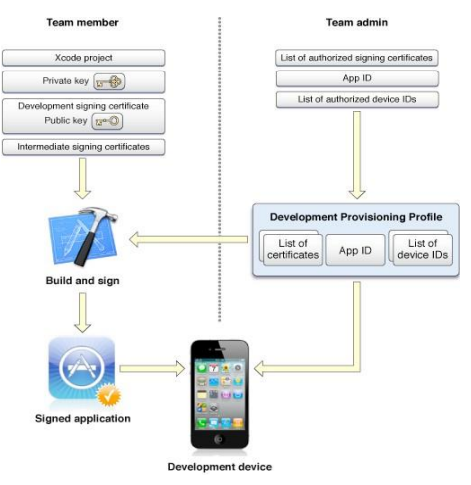
\includegraphics[width=0.75\textwidth]{graphics/iosAppDevelopmentProvisioningProfiles}
\end{figure}

\subsubsection{App Store deployment}
Apple certifies and signs the app bundle (executable, resources, etc.) App ID and no device information. Trust is based on Apple's certificate. iOS ships with root anchors for certificate chains.\\

There is no need for antivirus apps on iOS as Apple checks the app before distribution.

\subsubsection*{Certificate Revocation}
Apple supports revocation through
\begin{itemize}
    \item \textbf{Certificate Revocation List (CRL).} Server holds a list of revoked certificates
    \item \textbf{Online Certificate Status Protocol (OCSP)}
\end{itemize}

\subsubsection*{Sideloading in iOS}
Developers can release open source apps out of the App Store. Interested users can compile it in Xcode and run it on their own devices to bypass the App Store.\\

Compared to Android, it is much more complicated as it requires a physical connection to a Mac that has Xcode. The purpose of this is so that developers can test software on real hardware.


\subsection{Data execution prevention}
A \textbf{stack overflow attack} occurs when a program writes to a memory address on the program's call stack outside of the intended data structure, which is usually a fixed-length buffer.

\begin{lstlisting}
A()
{
   B(5);
   printf("done");
}

B(int a)
{
   char name[5];
   gets(name);
}
\end{lstlisting}
If the value of \texttt{name} is larger than 5 characters, it starts to corrupt the stack. If you pass in \texttt{
<nop><malware><addrs of name[1]>} you will overwrite the return address of \texttt{A()} to be the address of \texttt{name[1]} which is the location of the inserted malware.\\

\begin{figure}[h]
\centering
\caption{Stack Overflow Attack}
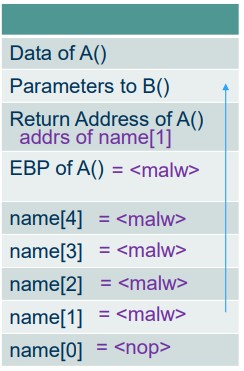
\includegraphics[width=0.4\textwidth]{graphics/stack}
\end{figure}

To prevent buffer overflow attacks, don't allow writable pages to be executable. \\

\paragraph{Data execution prevention} Executable pages are not writable. This prevents code modification (uses ARM NX bit on pages; never execute) and prevents dynamic production of code (except MobileSafari JIT code). All page requests and permission changes are checked.\\

DEP can be bypassed with \textbf{return-to-libc} exploits. With this, point return address to \texttt{system()} in libc. Call to \texttt{system()} is not allowed in iOS.\\

\textbf{Return oriented programming} was inspired by return-to-libc.


\subsubsection*{MobileSafari JIT}
DEP ruled out just-in-time (JIT) compiling, which is essential for making MobileSafari faster. A compromise was made - only MobileSafari is allowed to make writable and executable memory region. Only one such memory region is allowed. The checks only made in kernel at runtime. Malicious shell code can be written to JIT buffer area; so MobileSafari flaws can result in malware being injected.

\subsubsection*{Return-oriented programming}
Attacker gains control of call stack to hijack control flow and executes carefully chosen machine sequences (\textit{gadgets}) that are already present in machine's memory.\\

Each gadget typically ends in a return instruction and is located in a subroutine within existing program. They are chained together to perform actions.\\

ROP to disable DEP exists, but is ineffective in iOS due to code signing. In iOS, ROP payload should contain the malware but this is difficult.\\

For ROP to succeed, the memory addresses of an app in execution need to be found (in executable code, heap, stack).


\subsection{Address Space Layout Randomization (ASLR)}
Code signing and DEP are not sufficient to withstand ROP. \textbf{ASLR} randomizes the memory location (base address) of key program components. It was originally designed to overcome return-to-libc attacks.\\

ASLR works best if all code is compiled with the \textbf{position independent execution} (PIE) flag. Many third-party apps are not compiled for PIE.\\


\begin{figure}[h]
\centering
\caption{ASLR}
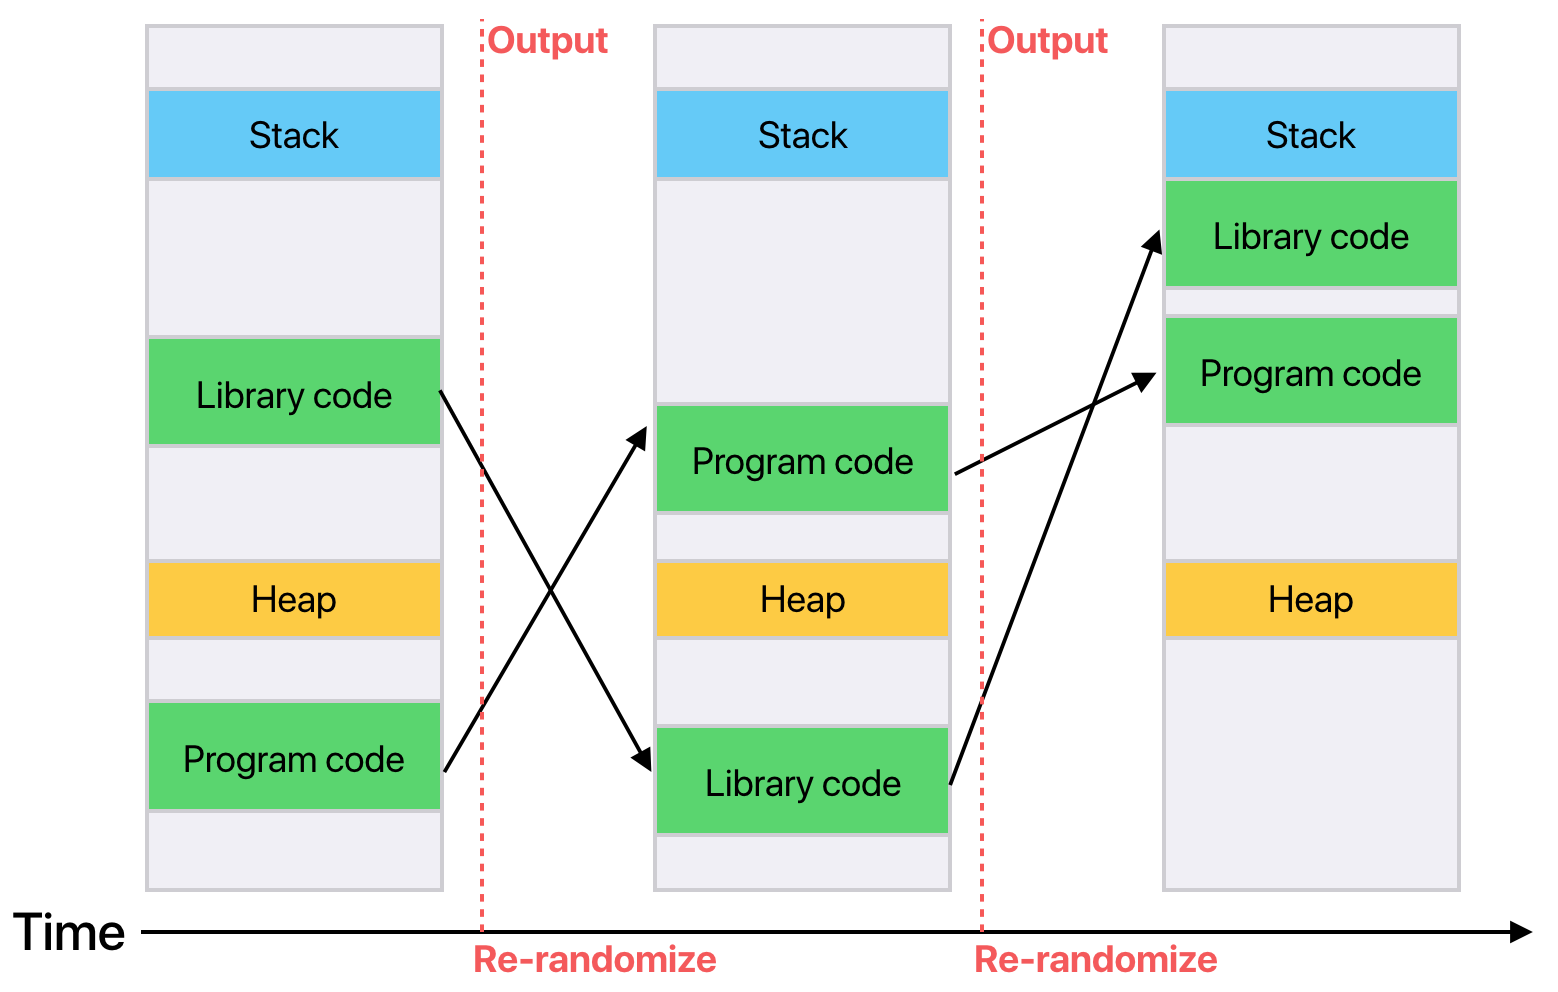
\includegraphics[width=0.7\textwidth]{graphics/aslr}
\end{figure}

\begin{figure}[h!]
\centering
\caption{Partial vs. full ASLR}
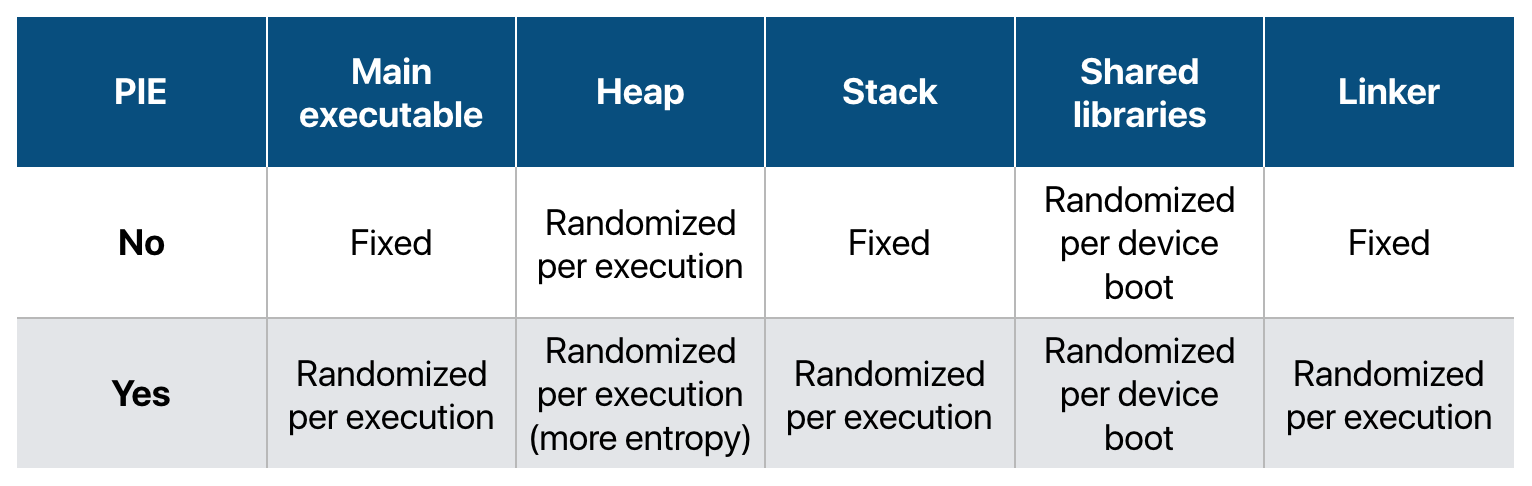
\includegraphics[width=0.9\textwidth]{graphics/aslrtable}
\end{figure}

\textbf{ASLR based on entropy.} Single non-randomized area can be enough for attacker. The larger the range of entropy (32/64-bit), the better. Relocation frequency is important as well (randomization during boot time vs. execution time).

\subsubsection*{Address Leakage}
Getting address information from an app. Brute force can be effective. Lots of exploits have been designed to leak addresses. PIE is not enough; we need every function/method scattered randomly through address space, or if we find one address we can determine others.\\

DEP and ASLR make it harder to mount attacks, but ASLR is still vulnerable to ROP with address leakage.

\subsubsection*{ASLR in iOS}
Introduced in iOS 4.3 and fully supported starting from iOS 5.

\subsubsection*{ASLR in Android}
Introduced in Android 4.0 and fully supported starting from Android 4.1. Android 5.0 dropped non-PIE support and required all dynamically linked binaries to be position independent.

\subsubsection*{Preventing malicious apps}
Static and dynamic analysis to prevent malicious apps at submission time. Prevent malicious apps at install/load-time through code signing enforcement (CSE). OS-level prevention with DEP and ASLR.

\subsection{iOS sandboxing}
DEP can be bypassed with the return-to-libc attack by overwriting the return address of a caller function with the address of the library function.\\

\paragraph{Sandboxing} Isolating app data and code execution from other apps so that if the app is compromised, its effect on other apps is minimized. Done through a set of fine-grained per-app-based access control that restricts app's access to resources (hardware, network, files, etc.)\\


Key idea: developer expresses what resources each app requires, and iOS allows/denies resources to the app. Each app runs in its own container (space in filesystem), and user controls access to documents.

\paragraph{Entitlements} Part of provisioning profile. Developers mentions what specific resources the app requires. One of them is enabling app sandboxing, which removes all but a minimal set of privileges. Other required privileges are restored one-by-one with appropriate entitlements.\\

\subsubsection*{App container}
An app's access to the file system is limited to container directories created during installation.
\begin{itemize}
	\item \textbf{iOS 8 and 9.} Container stored within \texttt{/var/mobile/Containers}
	\item \textbf{iOS 10.} Container stored within \texttt{var/Containers} 
\end{itemize}

Each container directory has a specific role. A \textbf{bundle} container is read-only, signed to prevent writing by user, and contains the app and its resources. The \textbf{data} container has various sub-directories to organize app's data.

What do container directories store?
\begin{itemize}
	\item \texttt{APPNAME.app/} The signed bundle with app code and static data
	\item \texttt{Documents/} App-specific user-created data files that can be shared through the File Sharing features in iTunes.
	\item \texttt{Library/} App support files.
	\item \texttt{Library/Preferences/} App-specific preference files.
	\item \texttt{Library/Caches/} App-specific data that should persist but don't need to be backed up.
	\item \texttt{tmp/} Temporary files that don't have to persist.
\end{itemize}

Entitlements are used to access outside files. They can be user selected files, or specific ones with programmatic access to standard locations:
\begin{itemize}
	\item \textbf{Downloads.} \texttt{com.apple.security.files.downloads.read-write}
	\item \textbf{Music.} \texttt{com.apple.security.assets.music.read-only} / ...\texttt{.read-write}
\end{itemize}

There are limited channels for sharing data outside of sandbox. Apps with the same \textbf{ApplicationIdentifierPrefix} can share data through the keychain (not just passwords now), as they are from the same developer. It's also possible to share data via servers or the clipboard.

\subsubsection{Sandbox implementation}
The sandbox is implemented as a policy module in TrustedBSD MACF.
\begin{itemize}
	\item Valid operations of a process are constituted as policies (and stored as a set of rules; a.k.a. profile)
	\item User space library functions to turn profile to system calls for installing and configuring sandbox
	\item A kernel extension (\texttt{sandbox.kext}) to evaluate policy restrictions and a kernel extension to enforce individual policies.
	\item A Mach server to handle logging from kernel and to hold prebuilt configurations.
\end{itemize}

\subsubsection*{Profile}
A \textbf{profile} is a set of per-process conditional rules defining access to system calls. Rules can require capabilities (entitlements, sandbox extension). It is written in Sandbox Profile Language (SBPL). \\

Each rule consists of a \textbf{decision} (e.g. deny), \textbf{operation\footnote{Seem symmetrical to MAC policy hooks.}} (e.g. file-read*), and \textbf{filter}\footnote{A filter includes a type and an optional value. Logical operations can be done through metafilters (require-all for AND, require-any for OR, and require-not for NOT; require-entitlement implies require-all.} (e.g. literal \texttt{/bin/a.txt}). SBPL code is compiled into binary blob graphs. There are built-in profiles for built-in apps, and a container sandbox profile for all third-party apps.\\

Stored as \textit{compiled binary blobs}, in \texttt{sandboxd} from iOS 5 to 8, and in \texttt{sandbox} kernel extension for iOS 2, 4, and from 9.\\

Until iOS 8, there is a different blob for a different sandbox profile. From iOS 9 onwards, there is a single binary blob.

\begin{figure}[h]
\centering
\caption{Sandbox overview}
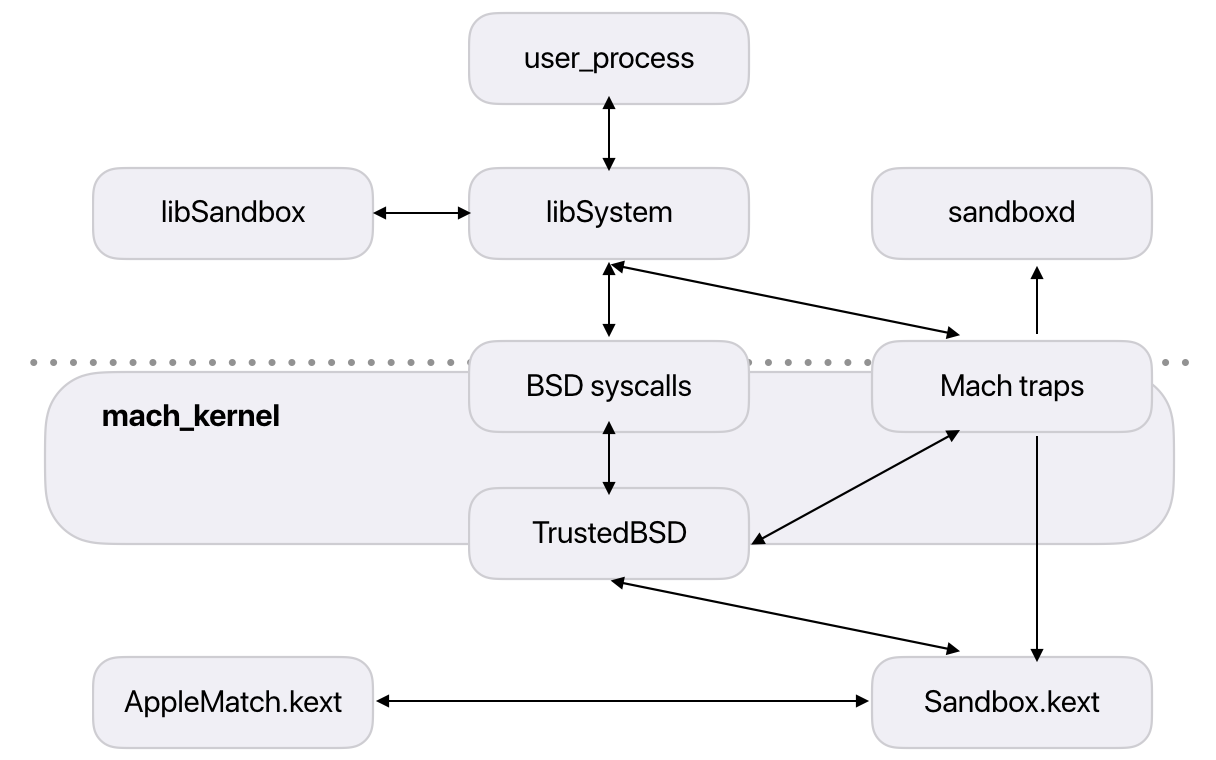
\includegraphics[width=0.75\textwidth]{graphics/sandbox}
\end{figure}

\subsubsection*{How does sandboxing work?}
Sandboxing begins with a call to \texttt{sandbox\_init}, a libSystem function by giving a profile as an argument. \texttt{sandbox\_init} uses \texttt{libSandbox} to convert the profile into a binary format that the kernel expects, which is passed to \texttt{mac\_syscall} and handled by the TrustedBSD subsystem.\\

TrustedBSD passes the sandbox initialization request to \texttt{Sandbox.kext}, which installs the sandbox profile rules for the current process. A return value is sent back when done.\\

When the sandbox is initialized, function calls hooked by TrustedBSD pass through \texttt{Sandbox.kext} for policy enforcement. It consults the list of rules for the current process, and for rules requiring pattern matching, functions from \texttt{AppleMatch.kext} are imported to perform regex matching.\\

\texttt{sandboxd} is used to carry tracing and logging info (and requests for prebuilt profiles.

\subsection{iOS encryption}
There is hardware support for encryption with a dedicated AES-256 crypto engine built into the DMA path between flash storage and main memory. There are two keys: a unique device ID (UID) and a device group ID (GID) fused to the chip. A random number generator is used to create other keys and a secure enclave manages keys. There is effaceable storage to securely erase keys.\\

The \textbf{Secure Enclave} is a virtual secure coprocessor. It communicates with application processor using interrupt-driven mailbox and shared memory data buffers.\\

Flash drive employs wear-leveling due to which multiple copies of data need to be deleted. Multiple copies are created when data erased frequently.\\ Block 0 of NAND as the \textbf{effaceable storage} and can be addressed directly and deleted surely.

\subsubsection*{Encryption}
\paragraph{Encrypt each file with a passcode.} Prone to brute-force attacks. Changing passcode will require re-encryption.\\

We can stretch passcodes using a \textbf{key derivation function} and get a secret passcode key from passcode.

\paragraph{Encrypt using passcode key.} Changing passcode still requires re-encryption of contents.

\paragraph{Encrypt each file with a file key and encrypt file key using passcode key.} Changing passcode only requires re-encryption of file key with the new passcode key.

\subsubsection*{Access control}
Some files should be accessible at any time; others should only be accessible when the device is unlocked. File protection classes via key hierarchy are used.

\begin{itemize}
	\item \texttt{NSFileProtection} \textbf{Complete.} File accessible when device is unlocked. Class key removed 10s after device locked automatically or manually. Useful for mobile banking.
	\item \texttt{NSFileProtection} \textbf{Complete Unless Open.} File can be created when device is locked but only accessible when device unlocked. Examples: mail attachments, photo/video.
	\item \texttt{NSFileProtection} \textbf{Complete Until First User Authentication.} Protected unless device is booted and user enters passcode for the first time. Example: SIM contacts.
	\item \texttt{NSFileProtection} \textbf{None.} File can be accessed at any time. Example: wallpaper.
\end{itemize}

\subsubsection*{Class key}
Different class keys represent circumstances under which files should be accessed. A file key is encrypted using a class key, and a hardware key and passcode key are used to protect class keys.\\


\begin{figure}[h]
\centering
\caption{Class Key}
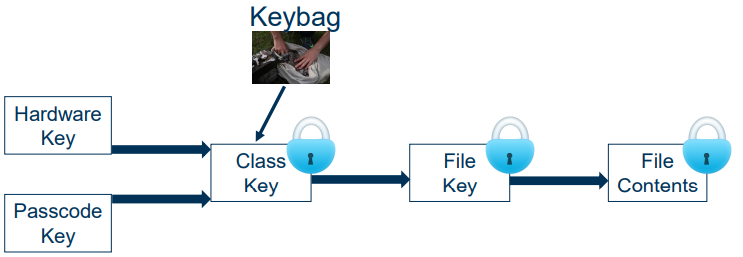
\includegraphics[width=0.75\textwidth]{graphics/classkey}
\end{figure}


Keys for file and keychain data protection classes are colected and managed in \textbf{keybags}. iOS has four keybags:
\begin{itemize}
	\item System keybag
	\item Backup keybag
	\item Escrow keybag
	\item iCloud backup keybag
\end{itemize}

The \textbf{UID} is an AES 256-bit hardware key unique to the device. It is in the secure enclave and cannot be accessed through software. This key encrypts a static string to produce the \textbf{hardware/device key}. This is not stored by Apple or its suppliers.

\begin{figure}[h]
\centering
\caption{Key Hierarchy}
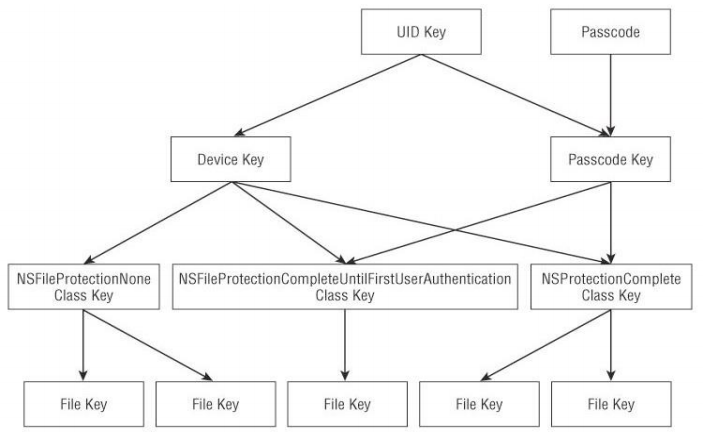
\includegraphics[width=0.9\textwidth]{graphics/keyhierarchy}
\end{figure}

\begin{figure}[h!]
\centering
\caption{Creating the File}
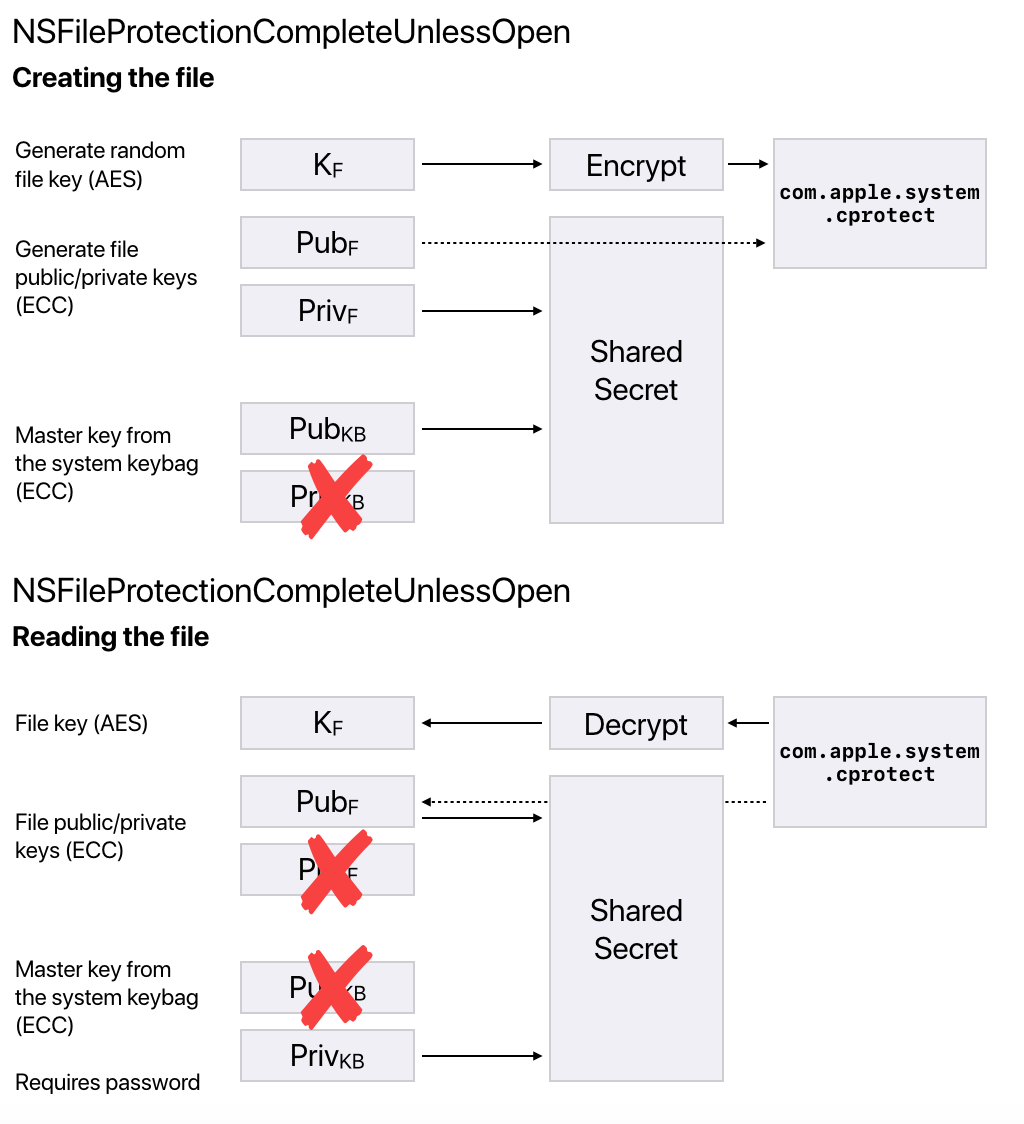
\includegraphics[width=0.95\textwidth]{graphics/completeunlessopen}
\end{figure}


\subsubsection*{File system key}
File system key encrypts file metadata. It's created when iOS is installed or when the device is wiped by the user. It is encrypted with the hardware key.\\

Encrypted file system key again encrypted by effaceable key (in effaceable storage) for quick erase.
\begin{figure}[h]
\centering
\caption{File System Key}
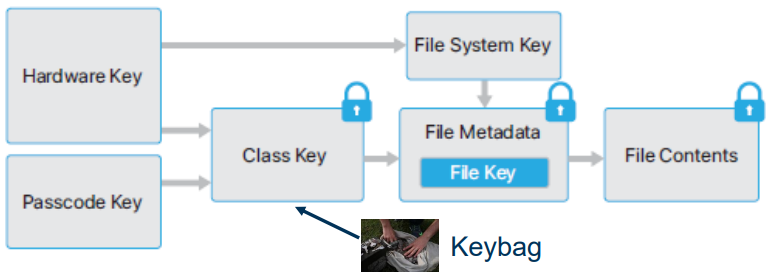
\includegraphics[width=0.75\textwidth]{graphics/filesystemkey}
\end{figure}

\begin{figure}[h]
\centering
\caption{Key Hierarchy}
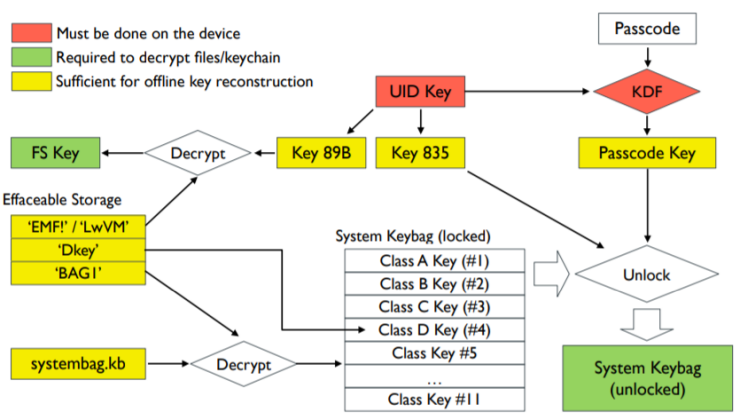
\includegraphics[width=0.75\textwidth]{graphics/keyhierarchy_2}
\end{figure}

\subsubsection*{Why layered keys?}
The entire filesystem can be rendered useless by wiping filesystem key. Modifying passcode just rewraps the class key. Changing a file's class only requires rewrapping file key. If device key is used, files or keychain items could only be restored using same device.\\

\subsubsection*{Keychain}
A \textbf{keychain} is a secure container to store short but sensitive data: passwords, keys, login tokens, etc. It is encrypted using 256-bit AES.\\

The \texttt{securityd} daemon determines which Keychain items each app can access. It uses access control lists to set policies for accessibility and authentication requirements.\\

Keychain items can be shared between apps of the same developer.\\

A class structure is used for protection:
\begin{itemize}
	\item \texttt{kSecAttrAccessible} \textbf{When Unlocked.} Accessed when device unlocked.
	\item \texttt{kSecAttrAccessible} \textbf{After First Unlock.} Protected unless passcode entered.
	\item \texttt{kSecAttrAccessible} \textbf{Always.} Not protected and always accessible (default).
\end{itemize}

For each of the above classes there is also a \textbf{This Device Only} variant which is non-migratory.

\subsection{iOS privacy}
\begin{itemize}
    \item Only you can access your device
    \item Your personal data belongs to you
    \begin{itemize}
        \item Apple does not sell your data to third-parties (except they do)
        \item Apple does not track what you shop (they probably do this as well)
    \end{itemize}
    \item Your experience improves while your data stays private
    \item Differential privacy - scramble data and mix it with other users so that the general pattern can be known but not specifics
    \item Apple does not want to know
    \begin{itemize}
        \item Which emoji you are using the most
        \item Which new word you introduced
    \end{itemize}
    \item Apple wants to know
    \begin{itemize}
        \item The most used emoji
        \item What new words are introduced
    \end{itemize}
    \item \textbf{Goal}: stronger privacy and rich user experience
\end{itemize}

\subsubsection*{Some Privacy Measures}
\begin{itemize}
    \item Identifiers
    \begin{itemize}
        \item Short-lived
        \item Random
        \item Anonymous
    \end{itemize}
    \item Data collection
    \begin{itemize}
        \item Bucket
        \item Sample
        \item Differential privacy
    \end{itemize}
\end{itemize}

\subsubsection*{Identifier API}
\begin{figure}[h]
\centering
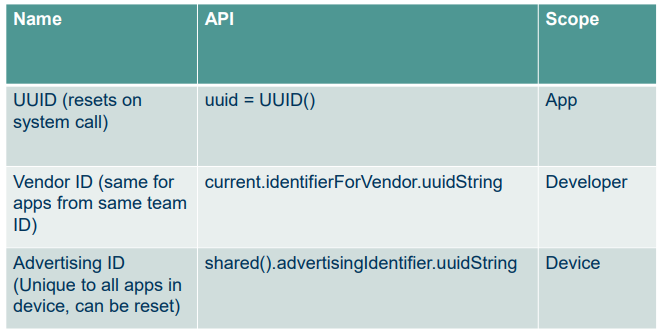
\includegraphics[width=0.75\textwidth]{graphics/identifierapi}
\end{figure}

\subsubsection{Differential Privacy}
\begin{itemize}
    \item A formal way of protecting individual privacy in a group by \textbf{adding noise}
    \item The results from the database with or without an individual must not disclose privacy information of the individual
    \item Add statistically biased noise to data bit which averages out over a large number of data points
    \item A randomized function F is $\epsilon$-differently private if for all data sets $D_{1}$ and $D_{2}$ differing at most by one element and all $S\subseteq Range(F)$
\end{itemize}

\begin{shaded}
$Pr[F(D_{1}\in S)] = e^{\epsilon} \times Pr[(F(D_{2} \in S)]$ where $e^{\epsilon} is 1 + \epsilon$
\end{shaded}

\paragraph{How Much Noise to Add?}
The probabilities of \textit{results with or without an individual} are almost the same. The noise should be a function of $\delta F$ and $\epsilon$

\subsubsection*{How to Generate Noise}
\begin{itemize}
    \item Noise = Random value from the distribution with standard deviation large enough to fill the gap
    \item Using probability distribution
    \item Type of distribution depends on F
    \item F is numeric - Laplace distribution
    \begin{itemize}
        \item $Lap(b) = \frac{1}{2b} exp (\frac{x}{b})$
        \item $Variance = 2b^{2}$
    \end{itemize}
    \item F is categorical - Exponential distribution
\end{itemize}

\subsubsection*{How it Works}
\begin{itemize}
    \item Hash the value so that it becomes a fixed length (125 -$>$ Hash -$>$ 00010100111001)
    \item Add noise by flipping some bits (000101001110001 -$>$ Add Noise - $>$ 010100001110000)
    \item By averaging all the values you will end up with the original hash
    \item The probability of changing 0 to 1 and 1 to 0 is less than the probability of unchanging 0 and 1
\end{itemize}

\subsection{Enterprise Security in iOS}
\subsubsection*{Enterprise Concerns}
\begin{itemize}
    \item Enterprises have to manage devices that may be used to access or store the sensitive enterprise data
    \item This introduces the new security risks e.g. Misplaced devices, lost devices, stolen devices
    \item Basically, the sensitive enterprise data could be at risk
\end{itemize}

\subsubsection*{Enterprise Needs}
\begin{itemize}
    \item Control over devices in a number of ways
    \begin{itemize}
        \item Configuring devices (auto-lock)
        \item Managing data and app restrictions (e.g. no access to camera)
        \item Applying rules (strong passcode, remote wipe)
    \end{itemize}
    \item Users can do unsafe things, so enterprise security can help avoid the issues in the case of BYOD
\end{itemize}

\subsubsection*{Naive Approach}
\begin{itemize}
    \item IT admins can do configurations manually
    \item Unfortunately, there are issues with manual configuration as it is \textit{labour-intensive} and \textit{error-prone}
\end{itemize}

\subsubsection{iOS Configuration Management}
\begin{itemize}
    \item iOS based devices are managed through the creation and installation of configuration profiles
    \item These profiles contain settings configured by an administrator for installation on a user's device
    \item Configuration profiles are centrally managed using
    \begin{itemize}
        \item Apple's iPhone Configuration Utility
        \item Mobile Device Management (MDM) System
    \end{itemize}
\end{itemize}

\subsubsection*{Configuration Profiles}
\begin{itemize}
    \item Used to ensure organisation security policy
    \item An XML property list file (plist)
    \item THe plist data may optionally be signed and encrypted
\end{itemize}

\subsubsection*{Profile Metadata}
\begin{itemize}
    \item The configuration profile metadata includes
    \begin{itemize}
        \item The human-readable name
        \item Description of the profile
        \item Creating organisation
        \item Other fields
    \end{itemize}
    \item The configuration payloads are the most important portions of the profile
\end{itemize}

\begin{figure}[h]
\centering
\caption{Configuration Profile Payload Types}
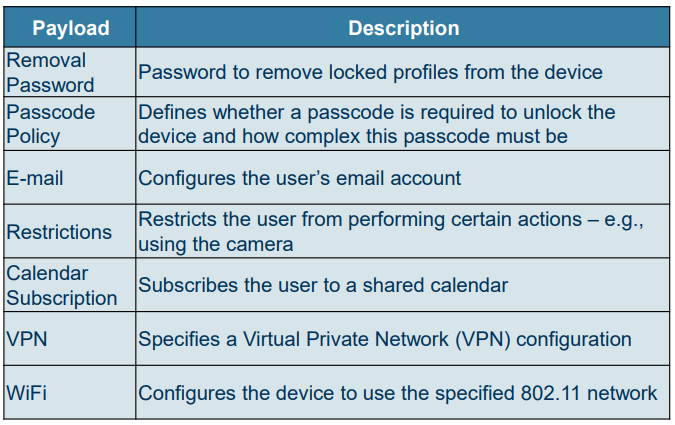
\includegraphics[width=0.75\textwidth]{graphics/configurationprofilepayloadtypes}
\end{figure}

\paragraph{Removal password} payload indicates the password needs to turn off the configuration profile. Configurations can also be set with 'Never Remove' - have to clear the device to get rid of it.

\paragraph{Passcode policy} specifies how complex a passcode should be. If there is no existing passcode or if it is not complex enough, then the user is asked to set a new passcode.

\subsubsection*{iPhone Configuration Utility}
\begin{itemize}
    \item A graphical utility for iPhone configuration
    \begin{itemize}
        \item It lets administrators create and manage configuration profiles
        \item Self-signed certificate created on the installing device at the first time of run
    \end{itemize}
    \item Installed onto iOS devices via USB connection
    \begin{itemize}
        \item Device specific certificates signed by the root certificate are automatically transferred to the iOS device for facilitating digital signature
    \end{itemize}
    \item Updated via USB, email or web server
    \item Issue: not scalable - only manages a limited number of devices
    \item Apple Configurator: More user friendly version of iPhone Configuration Utility
\end{itemize}

\begin{figure}[h]
\centering
\caption{Apple Configurator vs iPhone Configuration Utility}
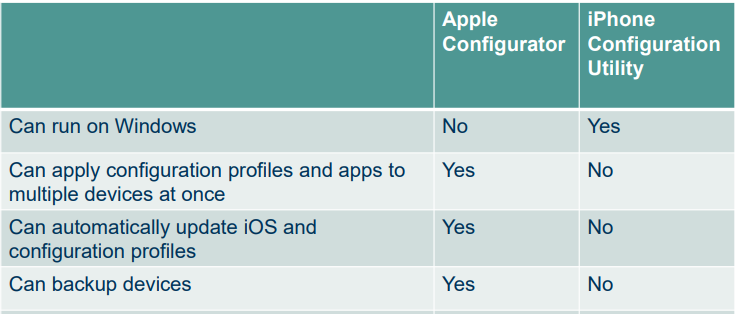
\includegraphics[width=0.75\textwidth]{graphics/appleconfigurator}
\end{figure}

\subsubsection{MDM Systems}
\begin{itemize}
    \item Used to manage a large number of devices
    \item Apple offers an MDM system in Lion server through the Profile Manager service
    \item The service works well for workgroups and SMEs
    \item For large organisations, a commercial third party MDM solution would likely work best
    \item 3 Components
    \begin{enumerate}
        \item iOS device
        \item Organisation's MDM server
        \item Apple's Push Notification Service (APNS)
    \end{enumerate}
\end{itemize}

\subsubsection*{How MDM Works}
\begin{itemize}
    \item Devices inform the APNS which topics they are subscribing to
    \item The MD server tells the APNS to publish a notification
    \item The notification is sent to the subscribed devices
    \item The device then establishes a connection to the MDM server over HTTPS
    \item A remote wipe command can be initiated by MDM, Exchange or iCloud
\end{itemize}

\subsubsection*{Enterprise Apps}
\begin{itemize}
    \item An enterprise provisioning profile can be loaded along with the configuration profile
    \item Then, the in-house enterprise apps can be distributed Over the Air (OTA) or through MDM
    \item Enterprise provisioning profiles have to be renewed annually
\end{itemize}

\subsubsection*{Kill Switch \& Hardware Modifications}
\begin{itemize}
    \item The kill switch worries some companies, what if Apple wants to shut our apps down?
    \item Some companies do not trust software restrictions - instead of relying on configuration profiles, companies can purchase special hardware
\end{itemize}

\subsection{iOS Jailbreaking}
\begin{itemize}
    \item Removing certain security restrictions, put by Apple, on iOS devices by manipulating the software stack
    \item Provides full access to the OS and filesystem
    \item Using installers like Cydia, it enables installation of apps and themes not approved by Apple
    \item Jailbreaking is legal in the United States - DMCA 2010 but can void the warranty
    \item People jailbreak their iOS devices for many reasons
    \begin{itemize}
        \item Install third-party software not supported by Apple
        \item An open platform for developing software
        \item To bypass cellular carrier locks
        \item To evaluate the security and discover vulnerabilities
    \end{itemize}
\end{itemize}

\begin{figure}[h]
\centering
\caption{iOS Chain of Trust}
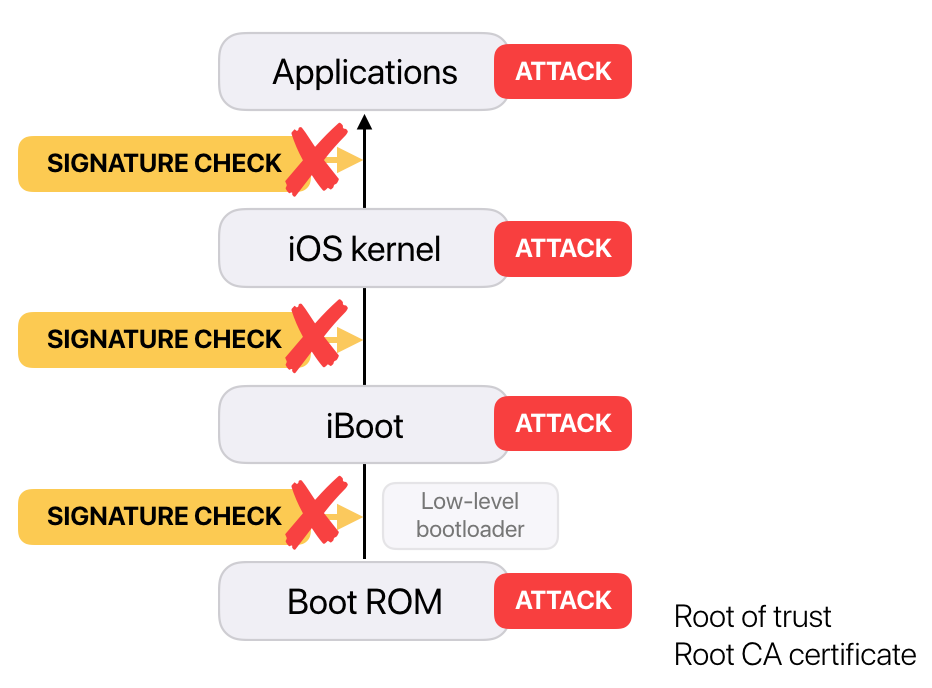
\includegraphics[width=0.5\textwidth]{graphics/chainoftrust}
\end{figure}

\subsubsection*{How to Jailbreak}
\begin{itemize}
    \item \textbf{Goal}: To be able to run unsigned code and change filesystem
    \item Bypass kernel-level checks
    \item \textbf{Attack using exploit}
    \begin{itemize}
        \item Buffer overflow
        \item ROP
        \item Disable DEP
    \end{itemize}
    \item \textbf{Kernel patch}
    \begin{itemize}
        \item Modifying file system
        \item Disabling code signing
        \item Changing behaviour of sandbox
        \item Disabling MAC policies
    \end{itemize}
\end{itemize}

\subsubsection{Exploit Types}
\begin{itemize}
    \item The location of a vulnerability impacts the access level
    \item Vary from the device hardware to its software
    \item There are three levels of exploits
    \begin{enumerate}
        \item Bootrom level
        \item iBoot level
        \item Userland level
    \end{enumerate}
\end{itemize}

\subsubsection*{Bootrom Level}
\begin{itemize}
    \item Vulnerabilities inside the hardware
    \item The most powerful vulnerabilities from the point of view of a jailbreaker (allows jailbreakers to modify the whole bootchain)
    \item Cannot be fixed by any software update
    \item Can be fixed only within the next hardware revision
    \item Famous exploits - SHAtter, Limera1n
\end{itemize}

\paragraph{Limera1n}is a heap-based buffer overflow in the USB Data Firmware Upgrade (DFU) stack of the bootrom
\begin{itemize}
    \item Connect the machine to a computer via USB
    \item Force into DFU mode
    \item User the overflow to run the code that can patch the signature verification code
    \begin{itemize}
        \item Boot of a ramdisk
        \item Run the patched version of the low-level bootloader and kernel
        \item These patches allow execution of unsigned code
    \end{itemize}
    \item This is only a tethered jailbreak but it can be used to create an untethered one
\end{itemize}

\subsubsection*{iBoot Level}
\begin{itemize}
    \item Vulnerabilities inside iBoot
    \item As powerful as that of the bootrom in terms of features - still early in the boot process
    \item Since iBoot is not baked into the hardware, they can be fixed by software upgrade
    \item Famous exploit - iH8sn0w (A5 iBoot exploit)
\end{itemize}

\subsubsection*{Userland Level}
\begin{itemize}
    \item Vulnerabilities in userland processes
    \item Less powerful
    \item Easier to fix
    \item These processes can run with any permissions
    \begin{itemize}
        \item Root user - system processes
        \item Mobile user - user applications
    \end{itemize}
    \item In both cases, at least two exploits required to jailbreak the device
    \begin{enumerate}
        \item Achieve arbitrary code execution
        \item Escalate privileges
    \end{enumerate}
\end{itemize}

\subsubsection{Kinds of Jailbreaks}
\begin{itemize}
    \item Depending on the vulnerabilities used, there are two kinds of jailbreaks with respect to jailbreak persistence
    \begin{itemize}
        \item Tethered jailbreaks: Disappears when the device is restarted (e.g. RedSn0w)
        \item Untethered jailbreaks: Permanent (e.g. pandora)
        \item Semi-tethered
        \item Semi-untethered
    \end{itemize}
\end{itemize}

\subsubsection*{Tethered Jailbreak}
\begin{itemize}
    \item The jailbreaks has to be enabled every time the device restarts
    \item The device has to be connected to a computer via a USB cable
    \item Kernel patched each time after reboot
    \item Exploit against privileged code (USB device driver)
    \item Exploit against unprivileged code + privilege escalation exploit
\end{itemize}

\subsubsection*{Untethered Jailbreak}
\begin{itemize}
    \item Permanent effect
    \item Harder to do because it needs to make permanent changes to the boot sequence
    \item Used to beasy when there was a vulnerability in the bootorm
    \item Now requires multiple exploits
    \begin{itemize}
        \item Start with a tethered jailbreak - unsigned code needs to be executed
        \item Find a way to install additional exploits on the root file system - privileges need to be escalated to patch the kernel
    \end{itemize}
\end{itemize}

\subsubsection{Jailbreakme 2.0 Star}
\begin{itemize}
    \item Userland exploit
    \item Go to the website and ajilbreak your phone without attaching it to a computer or rebooting
    \item Stack overflow when MobileSafari handled a particular font - the error was in the FreeType parser when rendering PDFs
    \item This allowed the exploit to mount ROP within MobileSafari
    \item This sophisticated payload proceeded to exploit another vulnerability to increase its level of access
    \item The second vulnerability was an integer overflow in an IOSurface property
    \begin{itemize}
        \item IOSurface is a private framework to share graphics between processes
        \item The second attack allowed code execution inside the kernel
    \end{itemize}
    \item From the kernel, disabled code signing
    \item The ROP downloaded an unsigned library that jailbroke the device
\end{itemize}

\subsubsection{Jailbreaking can be Dangerous}
\begin{itemize}
    \item Disables almost all security features
    \begin{itemize}
        \item Code signing - unsigned code can run
        \item Attack surface is increased
        \item Shell and other utilities added
        \item Can install root privileged code
        \item Unsigned apps are not sandboxed
    \end{itemize}
    \item Jailbreaking essentially reduces iOS security and makes devices vulnerable to different worms
    \item Example: Ikee worm
    \begin{itemize}
        \item Many jailbroken phones had an SSH Server installed
        \item Did not change the default root password \textit{alpine}
        \item SSH server was not sandboxed
        \item What did the worm do?
        \begin{itemize}
            \item Originally changed the wallpaper
            \item Later, it was used to lock the phone, steal contents and create botnets
        \end{itemize}
    \end{itemize}
\end{itemize}


\newpage
\section{Seminars}
\subsection{Stack Overflow Considered Harmful? The Impact of Copy \& Paste on Android Application Security}
\subsubsection*{[Fischer SP17]}
\textbf{StackOverflow} is a great place to get code snippets for all situations, including security-related situations. How safe is it to copy/paste such code into production software?

\subsubsection*{Grabbing code snippets}
\begin{enumerate}
	\item Download code from SO (all of them are in code tags)
	\item Determine if code is security related. Code is security related if it has calls to: \begin{itemize}
		\item Cryptography APIs
		\item Secure network communication APIs
		\item Public key infrastructure APIs
		\item Authentication/access control APIs
		\item BouncyCastle/SpongyCastle
		\item \texttt{HttpClient}
		\item Other libraries such as \texttt{jaspyt} or GNU Crypto
	\end{itemize}
	\item Classify code security. Manually analyze samples to train a machine learning algorithm (\textbf{Support Vector Machine}). 1360 snippets were classified.
\end{enumerate}

\begin{shaded}
\textbf{Code security}\\
\begin{multicols}{2}
Secure code snippets contained:
\begin{itemize}
	\item Good algorithm choice
	\item Secure length of keys
	\item Secure RNG
\end{itemize}
\vfill\null
\columnbreak

They were insecure if they had:
\begin{itemize}
\item Outdated algorithms
\item Static IVs/keys
\item Weak key lengths
\item Insecure RNG
\item Insecure TLS implementations	
\end{itemize}
\end{multicols}

\end{shaded}

Out of the 1360 snippets, 420 were insecure. This classifier was then applied to the rest of the snippets from questions and answers. 

\subsubsection*{Finding C/P code in real world apps}
The StackOverflow code was compiled into the same intermediate representation in DEX files with \textbf{WALA}. 85.2\% of answer snippets were converted. An exact match wasn't needed.\\

A program dependency graph (PDG) was made for each method. Data-independent subgraphs of a method are \textbf{semantic blocks}, and code similarity was given by the number of shared semantic blocks which share constants and method names. This process is automated.

\subsubsection*{Results}
\begin{itemize}
	\item Scraped over 4000 security related Android code snippets. About 30\% of them were insecure.
	\item Downloaded over 1.3 million free apps from the Play Store. 200k of them had SO code snippets; 196k (15\% of total) had at least one insecure snippet.
	\item The top offending snippet had to do with \texttt{TrustManager} with no server verification which could allow for MITM attacks.
\end{itemize}

\subsubsection*{Criticism}
Security is more than just algorithm and key-length. ML can't understand code yet so it could miss vulnerabilities. Code without context can result in an insecure labelling even if it's not used for security purposes.


\subsection{Cloak and Dagger: From Two Permissions to Complete Control of the UI Feedback Loop}
\subsubsection*{[Fratantonio SP17]}

The main point is to do malicious things to the user's phone without them being aware of it. Examples are: stealing logins, installing apps, clicking on ads, calling foreign numbers. This is done by \textbf{controlling the UI feedback loop} and manipulating what the user sees.

\begin{shaded}
\textbf{Dangerous permissions}\\

This vulnerability uses two Android permissions:
\begin{itemize}
	\item \texttt{SYSTEM\_ALERT\_WINDOW} is a permission that needs to be manually enabled but is automatically granted if downloaded from the Google Play Store. It is used to allow drawing over other apps' windows.
	\item \texttt{BIND\_ACCESSIBILITY\_SERVICE} is intended for accessibility-related apps. It can listen for click events and notifications in other apps, scroll and click for the user, and gives access to the full view tree. This isn't automatically granted but does not show up when installing. 
\end{itemize}

Both permissions are required for the attack. With only the first one, the attacker can modify what the user sees but can't react to their actions. With only the second one, the attacker can inject fake input but the user will know that they're being attacked.
\end{shaded}

\subsubsection*{Existing preventative measures}
If an overlay (from \texttt{SYSTEM\_ALERT\_WINDOW}) is being used as a \textbf{pass-through}, the app can't detect touches in its overlay. It is not possible then to overlay a transparent view and steal touches. However, it is possible to detect touches outside the overlay without coordinates (outside clicks set to (0,0)).\\

The \texttt{BIND\_ACCESSIBILITY\_SERVICE} permission needs to be explicitly enabled by the user and doesn't give access to passwords in the view tree.\\

\textbf{Clickjacking.} Apps can detect if a view is being overlaid, so instead we can overlay everything else and change the look of the overlay!\\ 

We can play a video in an overlay, and in the background install a malicious app and grant it permissions.\\

\subsubsection*{Keystroke inference}
We can read keystrokes with \texttt{SYSTEM\_ALERT\_WINDOW} by creating a passthrough overlay per key and stack them on each other. Each overlay has a flag to detect if it's being obscured, and to detect if an outside touch occurred. The lowest overlay that isn't obscured is the desired key. Overlays could also be used for fake login fields or ads.

\subsubsection*{User study}
20 university staff were asked to participate and install an app. None of them realized that they were being attacked; in the background an app was being installed.

\subsubsection*{Proposed fixes}
\begin{itemize}
	\item Allow apps to be marked \textbf{security-sensitive} so that they can't be drawn over. Don't let accessibility services click/enter text. (This would break apps like LastPass).
	\item Don't automatically grant \texttt{SYSTEM\_ALERT\_WINDOW}.
	\item Check apps that use both permissions.
	\item Display permissions at install-time.
\end{itemize}
From Android 8.0 onwards, apps can't draw over system views such as the notification bar. Notifications are also shown if an app is drawing an overlay.\\

Google is also limiting use of Accessibility Services for non-accessibility purposes.\\

Restricting overlays can be detrimental to user experience (chat heads!).

\subsection{The ART of App Compartmentalization: Compiler-based Library Privilege Separation on Stock Android}
\subsubsection*{[Huang CCS17]}
Developers use software libraries, such as platform libraries but also third-party libraries. Third-party libraries are used to either solve a problem (such as a physics engine), or for monetization (ad library/service).\\

Libraries run with the \textbf{same privileges} and in the \textbf{same sandbox} as the application. This could lead to data leakage and greater exposure to vulnerabilities. A library exploit could lead to an exploit in the app.\\

\begin{figure}[h!]
\centering
\caption{System overview of CompARTist}
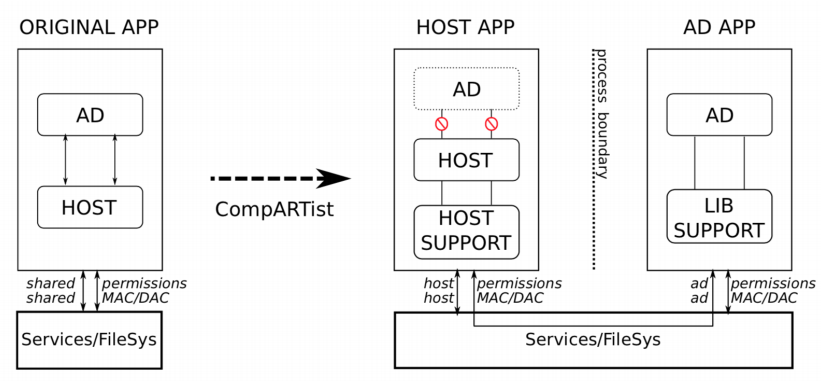
\includegraphics[width=0.9\textwidth]{graphics/compartment}
\end{figure}

The solution is to move the library into its own sandbox and to interconnect it with the host application with the Binder.\\

\subsubsection*{IPC}
Libraries rarely implement \texttt{Parcelable}, so transferring the original classes isn't an option. Authors implement \texttt{WrapClass} that is used by \texttt{AdHelper} to replicate access to objects to the other end.
\begin{figure}[h!]
\centering
\caption{Inter-application communication channel}
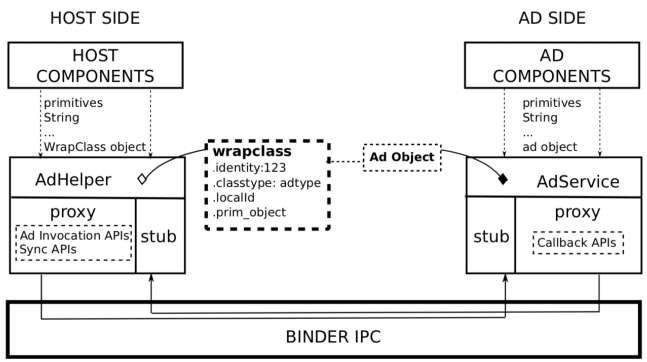
\includegraphics[width=0.7\textwidth]{graphics/IACC}
\end{figure}

The idea is to rewrite the app code during compilations to use \texttt{AdHelper} and IPC. First, entry points must be identified, then rewrite the code by traversing entry points down the call graph. Finally, the \texttt{AdHelper} library is injected.\\

In short, the app is split into a host and the ad app. IPC is used as communication between the two apps. Instrumentation replaces calls to the third-party library with calls to \texttt{AdHelper} that calls the ad app. Layout synchronization replicates GUI state.\\

Start-up is slow because IPC has to be initialized.

\subsubsection*{Criticisms}
This approach works for loosely coupled libraries, but would have high performance overhead for tightly coupled libraries.\\

This requires root privileges to replace the \texttt{OAT} files in the original app.\\

Advertisement companies might not care?



\subsection{Unleashing the Walking Dead: Understanding Cross-App Remote Infections on Mobile WebViews}
\subsubsection*{[Li CCS17]}
A \textbf{WebView} is an in-app browser that runs in the current app to load some content. This is convenient for users. When a URL in an app is triggered, it sends an intent to another app which redirects its WebView to load the URL content.\\

An \textbf{intent} is an abstract description of an operation to be performed.\\

Cross-app webview navigation (XAWN) can be intent-based through an \textbf{implicit scheme} (locates targeted apps through intent) or an \textbf{explicit scheme} (targeted towards a specific app). \textbf{Deep linking} links to a specific location within an app.\\

\subsubsection*{The Problem}
Navigations aren't guarded extensively by the mobile OS. They are protected solely on intent permissions and filters.\\

Security for WebViews are difficult to implement. Android provides domain controlling methods such as \texttt{shouldOverrideUrlLoading()} and \texttt{onPageStarted()} but they can be circumvented\\

XAWN weakness exploited through transition of apps.

\subsubsection*{Cross-App WebView infection}
This attack attempts to gain control, privileges, and user information of the hosting application. The attack infects the entry point app and then spreads from the remote adversary.

\paragraph{Phishing} Attempt to obtain sensitive information by disguising as a trustworthy entity in electronic communication.

\paragraph{Remote Deep Phishing} Facebook has a URL bar to show source of web content, so phishing can't take place. Twitter doesn't, so by infecting the Twitter UI, the app can display a fake login UI to impersonate Facebook.\\

When the user opens Facebook, the app isn't displayed but the infected WebView instantly invokes Twitter's WebView with a phishing login page. Once the user ``logs in,'' Facebook's main activity is displayed.

\paragraph{Remove Privilege Escalation} Install malware and sends messages without user consent after clicking a link.

\subsubsection*{Solution}
\textbf{ViewFinder} is a simple fuzzing system that scans apps for remotely-controllable WebView instances. Its code and manifest files are checked to find malicious intents. Out of 5000 apps, 7.4\% of them that receive intents from other apps were found to have vulnerable WebViews.\\

\textbf{NaviGuard} identifies and controls anomalous cross-WebView navigation requests. It prevents navigation without user permission and notifies users about the automated navigation.

\subsubsection*{Criticisms}
Apps were challenging to use. NaviGuard was only tested on a specific model.

\subsection{Hindsight: Understanding the Evolution of UI Vulnerabilities in Mobile Browsers}
\subsubsection*{[Luo CCS17]}
Are mobile web browsers becoming more secure when compared with older versions?\\

\textbf{Attack building blocks (ABB)} are different types of UI attacks. 
\begin{itemize}
	\item \textbf{Event routing.} Overlapping elements belonging to different origins used to reroute the user. Clickjacking is an example.
	\item \textbf{Limited screen real-estate.} Hiding address bars or rendering them differently. This can be dangerous as the address bar is needed to identify the website.
	\item \textbf{Security indicators and content.} There should be indicators shown when a site has content other than HTTPS or when its certificate is signed by trustworthy authorities.
\end{itemize}

The test was done testing each ABB using Hindsight, as manual testing would be time consuming. Web browsers were found from Google Play, and older versions were found through third-party sites. Some browsers that didn't work were removed, and others that didn't work with Hindsight due to there being a splash screen were also filtered out.\\

Hindsight is an agnostic testing vulnerability framework. It can accommodate for all browsers, but due to differing layouts in some, it would not be possible to determine where the address bar is for some browsers. It used OCR to identify some elements.\\

98.6\% of browsers tested were vulnerable to at least one ABB attack. Half of the APKs were vulnerable to more than 12 (out of 27) ABBs. Browsers are becoming less and less secure. Popular browsers are more vulnerable than less-known browsers.

\subsection{A Stitch in Time: Supporting Android Developers in Writing Secure Code}
\subsubsection*{[Nguyen CCS17]}
There are many apps on the Play Store and developers fail to adhere to security best practices. This could be because of their inexperience/lack of security knowledge, their adoption of insecure practices, or just due to them using copy/paste.\\

Existing security tools require certain levels of security expertise to use. Android Lint doesn't, but doesn't emphasize security warnings and have limited data flow analysis functionality.\\

\textbf{FixDroid} is a static analysis tool based on Lint. It highlights code with additional explanations. It has a security indicator icon as well as suggests quick-fix options. It matches pasted snippets against an online database of known insecure snippets.\\

Students were given tasks. There was no significant difference in functional correctness but a difference in security success.

\subsubsection*{Criticisms}
\begin{itemize}
	\item Can it handle non-trivial tasks?
	\item Can it impact security?
	\item Only covers specific pitfalls.
	\item Not representative of all developers
\end{itemize}
\subsection{The Long-Standing Privacy Debate: Mobile Websites vs. Mobile Apps}
\subsubsection*{[Papadopoulos WWW17]}
Most online services offer both a mobile-friendly website and an app. Both are offered for free with revenue coming from ads. Ads may raise privacy concerns for users.\\

Websites track users through cookies. Cookie synchronization can be used to bypass the same-origin policy when collecting data. Ad libraries are embedded in applications, and also inherit the original app's permissions.\\

Data that could be leaked include personally identifiable information (PII) and device-specific identifiers (location, list of apps installed, etc.; this allows tracking without deletable cookies).\\

Selenium was used to automate collection of apps to form a dataset. The apps chosen were from the top 300 services ranked by Alexa. The dataset consisted of 116 sites and their apps from Alexa's top 300. LibRadar was used to detect embedded ad libraries.\\

Testing was done with a Raspberry Pi 2 to monitor outgoing resources. SSL sessions were monitored and traces are forwarded to a module for analysis.\\

56.67\% of apps contained a third-party ad library.\\

Location data leaked by 66\% of apps and 85\% of websites. Unique device IDs were leaked by many apps, allowing leaked data to be linked between apps. List of installed apps leaked by 3.45\% of apps, allowing profiling of user.\\

Chrome and Firefox don't leak unexpected identifiers, but sent a request to tracking domains while fetching google.com.\\

Apps are more prone to leak device ID information. \textbf{antiTrackDroid} is a tool that filters outgoing requests and blocks ones delivering tracking information, but requires the Xposed framework.
\subsection{WindowGuard: Systemic Protection of GUI Security in Android}
\subsubsection*{[Ren NDSS17]}
The Android GUI is comprised of many services, including \textbf{Activity Manager Service} and \textbf{Windows Manager Service}. An \textbf{activity} is a type of app component that provides at least one window. The AMS contains instance of each activity.\\

A \textbf{window} is a visual area on screen that shows the GUI. The WMS contains instance of each window (size, location, z-order, etc.). There are three types: app (associated with activity), system (special purpose), and sub-window.

\subsubsection*{Background}
How app's activity manages to display its window on screen:
\begin{enumerate}
	\item AMS launches a new app activity.
	\item Activity creates a window and registers itself to WMS.
	\item WMS asks SurfaceFlinger for drawing surface. Handler passed to app.
	\item App draws window's view hierarchy. SurfaceFlinger notified once complete.
	\item SurfaceFlinger displays the final frame.
\end{enumerate}

Current security mechanisms:
\begin{itemize}
	\item \textbf{App sandboxing.} Isolates an app's graphic information.
	\item \textbf{Binder token.} Client authentication. System services to securely identify clients to prevent spoofing.
	\item \textbf{Permission screen.} Access control that grants app permissions.
\end{itemize}

\subsubsection*{Problem}
User session is unprotected -- this is a list of GUIs the user has visited. Mobile screens are small so it's hard to verify app identity. Apps are allowed to launch new activities, add high z-order windows, or modify other apps' back stacks.

\paragraph{Android Window Integrity} No app has permission to perform any operations that adversely affect the user session. The display owner is the app of the current focused display and is more privileged than other apps.\\

Validation of states and their legitimacy. Legitimacy of activity session: mismatch between back stack and activity session. Legitimacy of current visible windows: stop windows overlaying display owner windows except white-listed or those belonging to the display owner. Legitimacy of future windows: same check as before, and also watching for misuse of \texttt{onBackPressed()}.\\

\textbf{WindowGuard} is an implementation of AWI model, as an Xposed framework module. If a violation is detected, a notification is used to inform the user.\\

Successfully detects 12 GUI attacks with little performance overhead. There are some false positives and negatives. Requires rooted device.

\subsection{Multi-touch Authentication Using Hand Geometry and Behavioral Information}
\subsubsection*{[Song SP17]}
People use biometric authentication to replace traditional methods of authentication. Simple physiological biometric methods (fingerprints) are vulnerable, but behavioral biometric methods are uncontrollable.\\

TFST (touch with fingers straight and together) gestures make use of multiple fingers. This technique is resilient to different attacks:
\paragraph{Zero-effort attack} Attacker tries to authenticate by change without any knowledge.
\paragraph{Smudge attack} Attacker uses oily traces left on screen as a hint.
\paragraph{Shoulder surfing attack and combination} Attacker watches authentication process of the user
\paragraph{Statistical attack} Attacker uses knowledge obtained from group statistics.

\subsection{Malton: Towards On-Device Non-Invasive Mobile Malware Analysis for ART}
\subsubsection*{[Xue USENIX-Security17]}
There are over 750k Android malware apps in the first quarter of 2017. Current Android malware analysis tools either:
\begin{enumerate}
	\item focus on a specific layer,
	\item run in the emulator,
	\item modify the DVM or the ART compiler, or
	\item modify the target apps.
\end{enumerate}

Current malware can detect whether they're being run in an emulator or in debug mode. They also employ obfuscation to evade static analysis detection.\\

Malton is a tool with multi-layer monitoring, information flow tracking, and path exploration. \\

The test involved collecting samples based on analyzed samples. Malton detected some stealthy behaviors such as phone calls and native code loading. It stores collected information in log files.\\

Malton is based off Valgrind. Malware samples can eventually detect existence of Malton and stop executing.\\

In-memory optimization reduces the code that needs to be executed. This is semi-automated as analysts have to specify entry/exit points.

\subsection{Cracking Android Pattern Lock in Five Attempts}
\subsubsection*{[Ye NDSS17]}
Pattern lock is a method of unlocking Android phones where users have to draw a sequence on a 3-by-3 dot grid satisfying several constraints. Existing solutions to crack pattern locks depend on smudge attacks or minor Wi-Fi signal changes.\\

The attack has five main stages:
\begin{enumerate}
	\item \textbf{Filming and pre-processing.} Find segment of video with the unlocking process using spatial-temporal heuristics.
	\item \textbf{Track fingertip locations.} Use tracking-learning-detection algorithm to find the trajectory of the fingertips. This requires location of the fingertip as well as some part of the device to calibrate for camera shakes.
	\item \textbf{Filming angle transformation.} Use matrix transformations to show pattern in user perspective.
	\item \textbf{Identify and rank candidate patterns.} Identify patterns based on number of segments, line length, and slopes.
	\item \textbf{Test patterns.} People tend to start from left to right.
\end{enumerate}

Data collection showed that more complex patterns were easier to crack than simple patterns. A test was done where people submitted their patterns.\\

Camera shake can be tolerated. Filming gave better results than direct observation.

\subsection{Proximity Based IoT Device Authentication}
\subsubsection*{[Zhang INFOCOM17]}
Wi-Fi routers that need to authenticate devices usually do this through a pre-shared key (PSK). This isn't available on IoT devices without a keyboard/screen. IoT devices connect with smartphones to input PSK. There are vulnerabilities with this.\\

The solution is to use \textbf{received signal strength (RSS)}, or how well a smartphone hears a packet. Individual values aren't useful but RSS variation is.
\begin{itemize}
	\item \textbf{Fast-changing channel attenuation.} Constantly change distance between two devices.
	\item \textbf{Antenna polarization.} Two devices rotating relative to each other.
\end{itemize}

Proximity to the device is important.
\subsubsection*{Move2Auth protocol}
When the user wants to send a PSK to the IoT device, the IoT sends a random public key. The IoT also sends identical packets encrypted with a corresponding private key to the smartphone. The user performs a gesture in front of the IoT device.\\

The smartphone records the RSS of each packet and record values of sensor on the phone. Three checks are made:

\begin{enumerate}
	\item Is the RSS variation big enough? Does it exceed the threshold?
	\item RSS traces and sensor traces compared based on shape and timing to determine correlation.
	\item Decryption of received packets. Do contents match?
\end{enumerate}

Testing was done in twelve locations in a simulated office space.

\subsubsection*{Limitations}
Have to be in close proximity and can only use a few gestures types. Determining threshold for the protocol can be difficult.

\subsection{SmartGen: Exposing Server URLs of Mobile Apps with Selective Symbolic Execution}
\subsubsection*{[Zuo WWW17]}
There are millions of apps and many apps use the internet for additional functionalities. Users don't have to worry about URLs and connections - but some usage is not desired! There is an illusion that the concealed server URLs are unattackable, secure, and hidden.\\

Server URLs are hard to find even if you have a proxy server that listens for network requests. Activities aren't easily navigable by automated means as some fields may require input validation. Even by going through app manually to find URLs, it is not guaranteed that all hidden paths will be found.\\

Even if the app is decompiled, parameter constraints can be hidden (pattern matching, predicates, input length, field confirmation, etc.), and other problems such as obfuscation or data format recognition.\\

Static analysis is scalable but not effective. Dynamic analysis tools are powerful but tools are limited. Emulators are slow.\\

\textbf{Symbolic execution} is the replacement of fixed inputs with symbols. This is done in conjunction with taint analysis\footnote{A method to check which variables can be modified by user input.} to identify constraints on code execution.\\

SmartGen is a targeted symbolic execution-enabled tool that works at the UI and system level. It is fully automated and is scalable. It constructs an extended call graph (with Soot!) using static analysis, and traverses graph to find invocations of network message sending APIs. It then extracts corresponding path constraints and solves them using z3. Afterwards, it executes app using new dynamic runtime and generates request messages with server URLs.


\end{document}
